\documentclass[times, utf8, diplomski]{fer}
\usepackage{booktabs}
\usepackage{fontspec}                       % for non-ASCII characters, with xelatex
\usepackage[binary-units=true]{siunitx}     % this one's for formatting SI units
\usepackage{graphicx}                       % \
\usepackage{subcaption}                     % / these two are for subcaptions

% These packages are for writing pseudocode.
% For details, see:
%     https://tex.stackexchange.com/questions/229355/algorithm-algorithmic-algorithmicx-algorithm2e-algpseudocode-confused#230789
%
%\usepackage{algorithm}    % for the float `algorithm` environment
\usepackage{algorithmic}  % for the actual pseudocode
\usepackage[ruled]{algorithm2e}

\begin{document}

\thesisnumber{1763}

\title{Evolutionary Heuristics for Fault Injection Parameter Space Search}
\crotitle{Evolucijske heuristike za pretragu prostora parametara napada umetanjem pogreške}
\engtitle{Evolutionary Heuristics for Fault Injection parameter Space Search}

\author{Antun Maldini}

\maketitle

\izvornik

\zahvala{}

\tableofcontents


% Questions for the introduction:
% -------------------------------
% what is the problem
% why is it interesting and important
% why is it difficult
% what have other people done
% what are the elements of our solution

% Structure:
% ==========
%   - motivation; twofold:
%      * stuff on cryptography, fault injection/analysis, EMFI in particular, which leads us to...
%      * the need for a better way to search the parameter space
% 
%   - related work: what have others done?
% 
%   - preliminaries:
%      * general crypto? but minimized to what's used
%      * EdDSA?
%      * SHA-3
%      * genetic algorithms
% 
%   - the THING:
%      * what was the plan & the setup
%         + the algorithm
%         + the baseline
%         + how we measure
% 
%   - results
%   - future work



\chapter{Introduction}\label{ch:introduction}
%The field of cryptography is a big one. As it is with most such fields, it
%abounds with rabbit holes: if you pick any one thing to know in detail, you'll
%end up going in progressively more detail, until you realize you're in deep
%enough that it's hard to describe your position to someone still at the
%entrance.
The field of cryptography is a pretty large and well-developed one. As it is
with most such fields, doing anything of worth means going down a rabbit hole
into progressively greater and greater detail, until it becomes hard to describe
where you are to someone standing on the surface. \\
This thesis is an attempt at covering one particular path down the rabbit hole.

Its structure is roughly this:
\begin{description}
    \item[Chapter~\ref{ch:introduction}] lays out the general motivation and
          the current state of the art;
    \item[Chapter~\ref{ch:prerequisites}] contains some technical prerequisites,
          covering evolutionary algorithms (and genetic algorithms in particular),
          fault injection, and SHA-3;
    \item[Chapter~\ref{ch:fault_injection}] presents the setup I've used and
          describes the parameter space and the problem at hand;
    \item[Chapter~\ref{ch:optimization}] deals with the optimization algorithm,
          the simulator built to aid experimentation, and the results obtained;
    \item[Chapter~\ref{ch:attacking_keccak}] presents the procedure of exploiting
          the faulty outputs, and covers the exploitation part of the results
    \item[Chapter~\ref{ch:conclusion}] just wraps it all up, and presents
          directions for future improvements.
\end{description}


\section{Motivation}
Cryptography is ubiquitous; as technology keeps advancing, the normal functioning
of key infrastructure now depends on cryptographic algorithms. Billions of people
worldwide rely on it daily to protect not only commerce, but also their privacy.
But even with good cryptographic primitives, new attacks keep being discovered,
commonly against implementations.

Zooming into this picture for something more concrete, we may find a service
provider running attacker's code on the same machine as a vulnerable encryption
library, just waiting for a cache-timing side-channel attack; or a TLS
implementation that will curteously say when the padding is wrong, thus letting
an attacker steal a session; or perhaps, a smartcard that can be persuaded by a
carefully placed glitch in its power supply to give out its secret PIN.

Surely, no one would want their bank account emptied just because someone had
physical access to their debit card. But attacks like these do exists, and it's
this last case that's most relevant for this thesis: fault attacks.

They're usually not the easiest thing to do, and one part of \emph{why?} is
picking the right parameters. The core part of this thesis concerns finding
a good algorithm for picking the parameters, and (if possible) mounting a
successful fault attack.


%Implementation attacks do not aim at the weakness of an algorithm, but at the
%weaknesses in its implementation instead. Two well-known kinds of implementation
%attacks are side-channel attacks (SCAs) and fault injection (FI) attacks.
%Side-channel attacks are passive, non-invasive attacks where the device under
%attack operates within specified conditions and the attacker simply observes
%the physical leakages produced. Fault injection attacks are, on the other hand,
%active, more invasive attacks where the attacker inserts faults (glitches) in
%order to disrupt the normal behaviour of the algorithm.
%
%Side-channel attacks received a lot of attention in the last few decades where
%we saw successful exploitation of several side channels like timing~\cite{kocher-timing_attacks},
%power consumption~\cite{Kocher_SCA}, and EM emanation~\cite{10.1007/3-540-45418-7_17}.
%To use that information and deliver as powerful as possible attacks, researchers
%devised various strategies. What is especially interesting is that many of those
%strategies in the last few years are based on machine learning~\cite{lerman11, PicekHJLGJM17}
%and deep learning~\cite{CagliDP17}.
%%Although considering distinct attack scenarios and often various techniques,
%%all those papers have in common that they establish different use cases where
%%machine learning is a powerful attack technique.
%
%Somewhat surprisingly, when considering fault injection attacks, the situation
%looks much more straightforward. There are  several sources of glitches like
%laser pulses, electrical glitches, and electromagnetic radiation. A fault
%injection attack is successful if after exposing the device under attack to a
%specially crafted external interference, the device shows an unexpected behaviour
%i.e. a fault, which can be exploited by an attacker. Here, the challenge lies in
%selecting the appropriate parameters for a fault to succeed. If those parameters
%are not well chosen, the target will respond in a way that does not permit an
%actual fault analysis attack. When considering various sources of faults, there
%are different number of parameters and corresponding ranges. In general, the
%search space size of possible parameter values is large and relatively few
%points in the search space result in faults. Consequently, an interesting
%question is: how to find suitable parameter values or intervals, or more
%precisely, how to efficiently find the correct values in the search space?
%Surprisingly, the main options today are to use either random search or some
%sort of exhaustive search (since full exhaustive search is usually not possible
%the attacker will concentrate only in some regions with a certain precision,
%which we call here grid search). Analogously, if it is possible to make SCA
%more powerful by using machine learning (and more generally, artificial
%intelligence) one would expect the same to be possible with the fault injection.

%In this paper, we discuss how to use a special type of metaheuristics called
%genetic algorithms in order to find parameter values resulting in faults for
%electromagnetic fault injection. A somewhat similar research direction is
%followed in several papers~\cite{10.1007/978-3-319-08302-5_16, 6859734, 10.1007/978-3-319-21476-4_11}
%but there the authors consider power glitching, which is a much simpler case
%from the search space size perspective, and they attack the PIN mechanism in a
%smartcard. Here, we use the faults obtained via our technique to mount an
%algebraic fault attack on a SHA-3 implementation where we consider only pulsed
%EMFI and we have a total of 5 parameters. We emphasize that our version of
%search algorithm differs significantly from previous works as detailed in the
%rest of the paper. Finally, our code is available as an open source implementation~\cite{memfaultsGithub}.\\


This thesis is partly based on~\cite{paper_FDTC2018}, and hence reuses some
of the material.

\section{Related work}\label{sec:related_work}
While a lot of work has been done on fault injection itself (see
e.g.,~\cite{Kommerling, boneh_demillo_lipton, nsamwel_africacrypt, impeccable_circuits, FI_crowbars}),
very little of it concerns parameter optimization.

In~\cite{madau2017fault}, the authors develop an EMFI susceptibility criterion,
which they use to rank the points of the chip surface depending on how susceptible
they are to fault injection. The underlying assumption for the criterion is the
Sampling Fault Model, described in~\cite{ordas2015injection}. The Sampling Fault
Model could be summarized thus: faults are (mostly) induced by violating the
setup time constraint of D-type flip-flops, and the length of the time window
for fault injection does not depend on the clock frequency. (Early on during
development, I considered this might provide a way to substantially decrease
the search space size in the time-offset dimension; the practical problems of
synchronizing to the internal clock and the comparatively low time resolution
of the equipment ensured that this direction was not pursued.) The criterion
itself is a combination of Power Spectral Density (measuring emitted power at
the clock frequency) and Magnitude Squared Incoherence (measuring how linked
the emitted signal is to the data being processed), weighted with a configurable
parameter $a$ like so:
\[
    emfisc_{x,y} = \sqrt{a \cdot psdn_{x,y}^2   +   (1-a) \cdot incn_{x,y}^2}
\]
where $psdn$ and $incn$ are normalized Power Spectral Density and Magnitude
Squared Incoherence, respectively.


They use a grid scan (in the 2 spatial dimensions) to measure all the points
and rank them according to the criterion; a share $\alpha$ of the highest-ranking
points are kept for further scanning; the rest is thrown away.
They are able to reject over 50\% of the chip surface (75\% in their best case),
while keeping 80\% of the points causing faults. Figure \ref{fig:emfisc} shows
their coverage ratio -- the share of preserved faulty points -- dependent on $\alpha$.
However, note that by \emph{fault}, they mean \emph{any} perturbation of the
normal behavior of the algorithm.

\begin{figure}[htb]
    \centering
    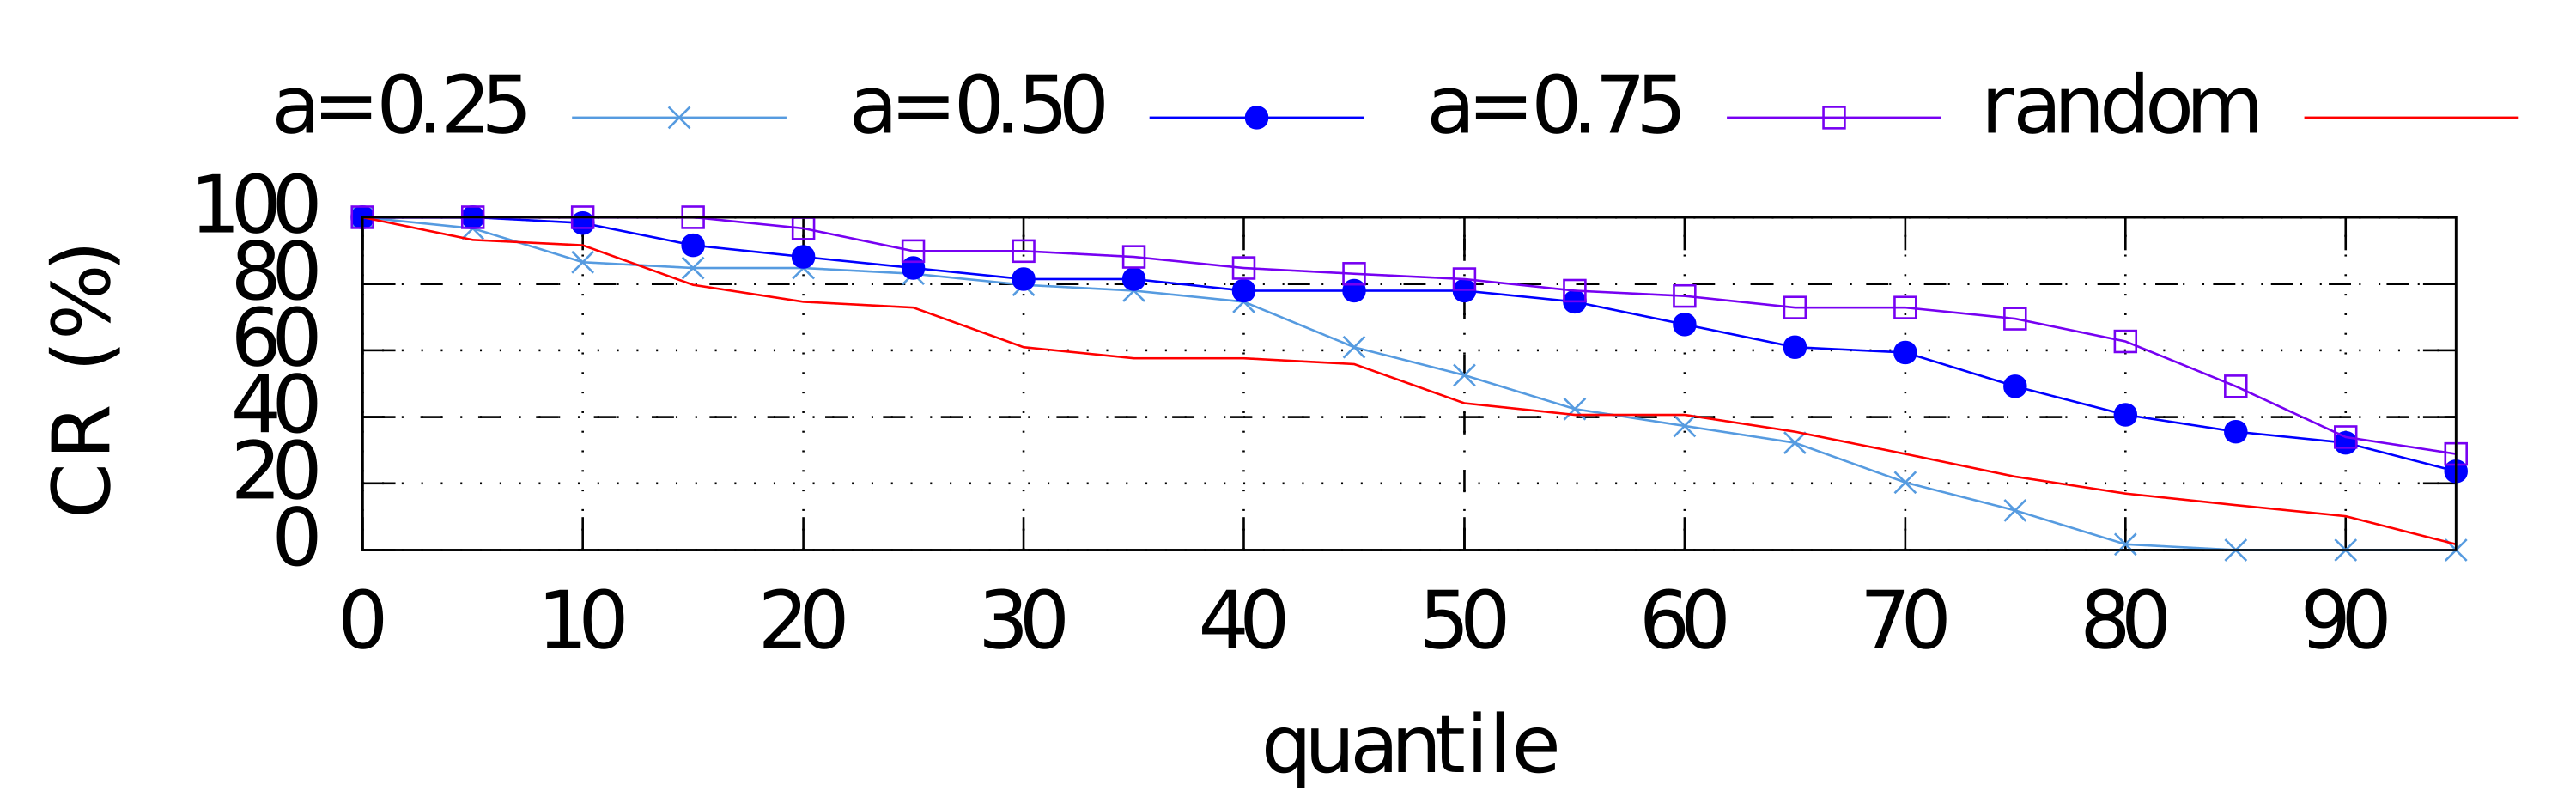
\includegraphics{images/emfisc.png}
    \caption{coverage ratio vs. $\alpha$ for EMFISC}
    \label{fig:emfisc}
\end{figure}


In~\cite{GlitchItIfYouCan}, the authors use several different methods to the
problem of parameter optimization for supply voltage (VCC) glitching. They work
with 3 parameters: glitch voltage, glitch length, and time offset. They reduce
the dimensionality of the problem by splitting the search in two stages,
effectively solving a "2.5-dimensional" problem, so to say. In the first stage,
they look for the best (glitch voltage, glitch length) combination, i.e. the
most promising shape of the glitch. All parameters not explicitly specified
 -- in this case, time offset and the number of glitch repetitions -- are
set as random. In the second stage, 10 most promising (voltage, length)
combinations are tried at each point in the specified time range (which is
discretized into 100 instants), i.e. they perform a grid search in the time
offset dimension.

The methods are compared at the first stage -- random search, FastBoxing and
Adaptive zoom\&bound algorithms, and a genetic algorithm. While Adaptive
zoom\&bound comes out as the best strategy of these, the genetic algorithm
shows some promise. 
%This approach is a ``smart'' search in 2D with a grid search in 1D.

That work is extended in~\cite{FI_memetic} where the authors use a combination of
genetic algorithm and local search (called a memetic algorithm) in order to find
faults even more efficiently. The authors consider power glitching with 3
parameters and are interested in fast characterization of the search space.
%TODO: describe FI_memetic more closely?


The evolutionary algorithm developed for the purpose of this thesis builds on
the ideas of the latter two papers.



\chapter{Prerequisites}\label{ch:prerequisites}
In order to understand what was done and how, several things must be understood
first. These are:
\begin{enumerate}
    \item genetic algorithms, used here for optimization
    \item fault injection (FI) in general
    \item the SHA-3 hash function, which is exploited here using algebraic fault analysis
    \item algebraic fault analysis (AFA), which is used in conducting a real attack
\end{enumerate}

SHA-3 and AFA are exposed first, so as to not interrupt the exposition of FI.


\section{SHA-3/Keccak}\label{sec:keccak}
In 2015., after a competition to choose the next SHA (Secure Hash Algorithm)
algorithm, NIST standardized Keccak~\cite{keccak_reference} as SHA-3.
Strictly speaking, SHA-3 is not one algorithm, but several, which all share
the same internal structure, and differ in a few parameters.

Its predecessors, SHA-1 and SHA-2, as well as some earlier algorithms which
weren't standardized but are still widely used (MD4, MD5), were based on the
Merkle-Damgård construction~\cite{merkle-damgard_revisited}. Figure \ref{fig:merkle-damgard}
shows the general concept: the algorithm operates on blocks of data of size $B$.
There exists an underlying function $f$, called the \emph{compression function},
which takes $2B$ bits of input and produces $B$ bits of output. $f$ is essentially
a small hash function itself, but one with fixed-length input and output, which
the Merkle-Damgård construction uses to build a "big" hash function, with
arbitrary-length input. It can be proven that the "big" hash function will
be collision-resistant if and only if the compression function is
collision-resistant~\cite{merkle-damgard_security}.

\begin{figure}[htb]\label{fig:merkle-damgard}
    \centering
    %TODO: 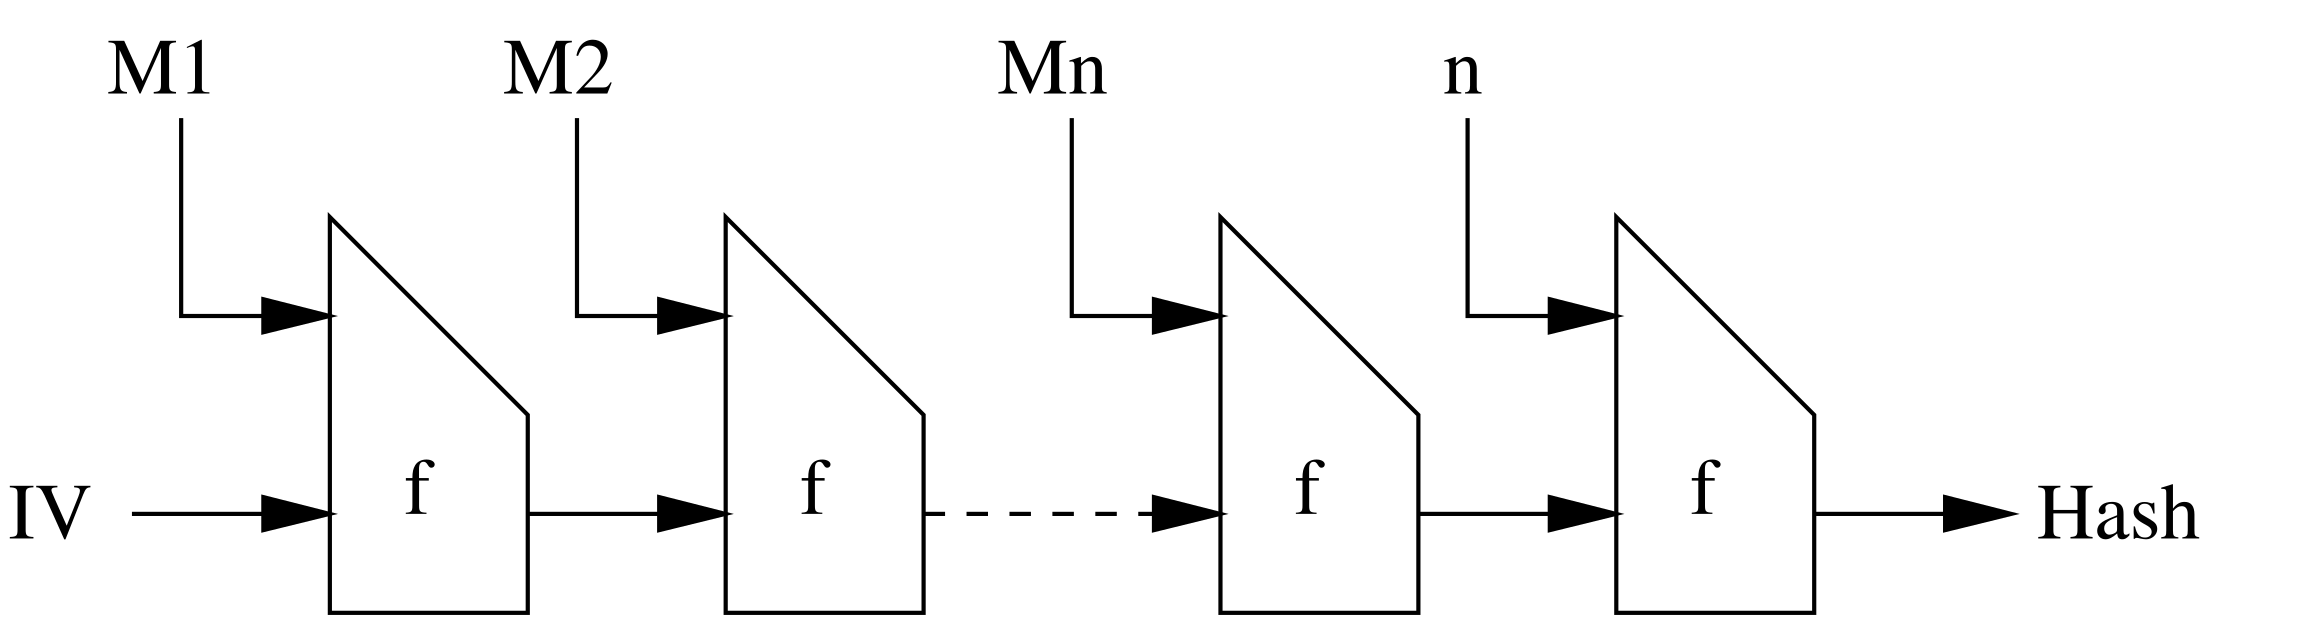
\includegraphics{images/merkle-damgard.png}
    \caption{the Merkle-Damgård construction}
\end{figure}


SHA-3, however, is based on a different construction called a \emph{sponge}.
It's called a sponge because unlike the Merkle-Damgård construction, which takes
an arbitrary amount of input and puts out a fixed-length output at the end, the
sponge can alternate between taking in chunks of input (\emph{absorbing}) and
putting out chunks of output (\emph{squeezing}); it has arbitrary-length output
as well as arbitrary-length input.
This is nicely illustrated in figure \ref{fig:sponge}.

%TODO: redo sponge description?
%TODO: take out sponge.png in better quality?

\begin{figure}[htb]
    \centering
    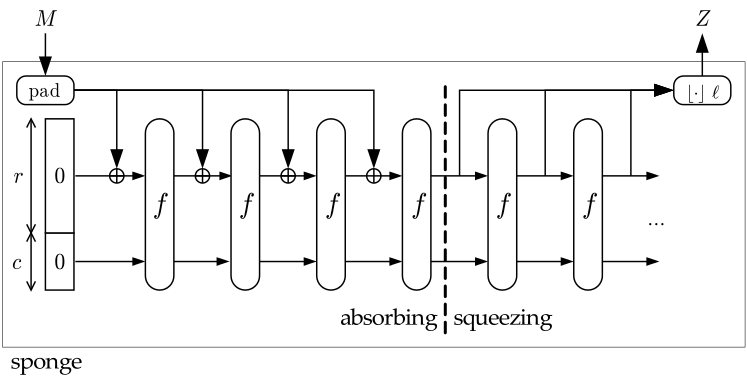
\includegraphics{images/sponge.png}
    \caption{the sponge construction}
    \label{fig:sponge}
\end{figure}

Another way to put it would be this: the Merkle-Damgård construction has a
compression function munging its internal state as well as chunks of input;
the sponge has a permutation mixing its internal state with chunks of input,
then mixing its internal state while spitting out chunks of output.

With traditional hash functions, security is expressed in terms of number of
output bits: a hash function with an $n$-bit output is supposed to have $n/2$
bits of security, i.e. the easiest attack has a complexity of $O(n/2)$.
This corresponds to having a random oracle output $n$ bits, and attacking it
with the generic attack which relies on the birthday paradox.

But here, expressing its security in such a way obviously wouldn't make sense:
with an arbitrary-length output, it would mean that we can get an arbitrarily
high level of security merely by squeezing more bits out of the sponge.
Instead, this is expressed as a single parameter of the sponge construction.


\subsection{The Keccak-$f[b]$ permutation}
The central part of the sponge construction is the permutation.
Keccak uses the Keccak-$f[b]$ permutation, where $b$ is the size of its internal
state; this is also called the \emph{width} of the permutation. In the variant
standardized as SHA-3, $b=1600$.
We define two parameters: \textbf{rate} ($r$) and \textbf{capacity} ($c$),
with the constraint that $r + c = b$. The sponge will absorb $r$ bits of input
for each invocation of the permutation by XOR-ing the chunk of input with the
first $r$ bits of the internal state; the rate essentially tells us how fast
is the input processed. The last $c$ bits of the state are never directly
touched from the outside, and are never output; the output is taken again from
the first $r$ bits of the state. Capacity is the single parameter that sums up
the security level: $c/2$ bits for collision resistance, $c$ bits for preimage
and second preimage resistance. Several concrete SHA-3 hash functions are
defined with different capacities, denoted SHA3-$c$: SHA3-224, SHA3-256,
SHA3-384, and SHA3-512. Only the last one, SHA3-512, will be considered in
this thesis.


And now, for the definition of the relevant variant of the permutation itself:
the Keccak-$f[1600]$ is a sequence of operations on a 1600-bit state $A$, which
we can represent as a three-dimensional array of bits: $A[5,5,64]$. Coordinates
$x$ and $y$ should be taken modulo 5 and coordinate $z$ should be taken modulo 64.
If an index is omitted, this means the statement is valid for all values of the
omitted indices, e.g. $A_{(x,z)}$ refers to the column of bits having coordinates
of the form $(x,\ast,z)$. Figure \ref{fig:keccak_state} shows the notation used
for different parts of the state.

\begin{figure}[htb]
    \centering
    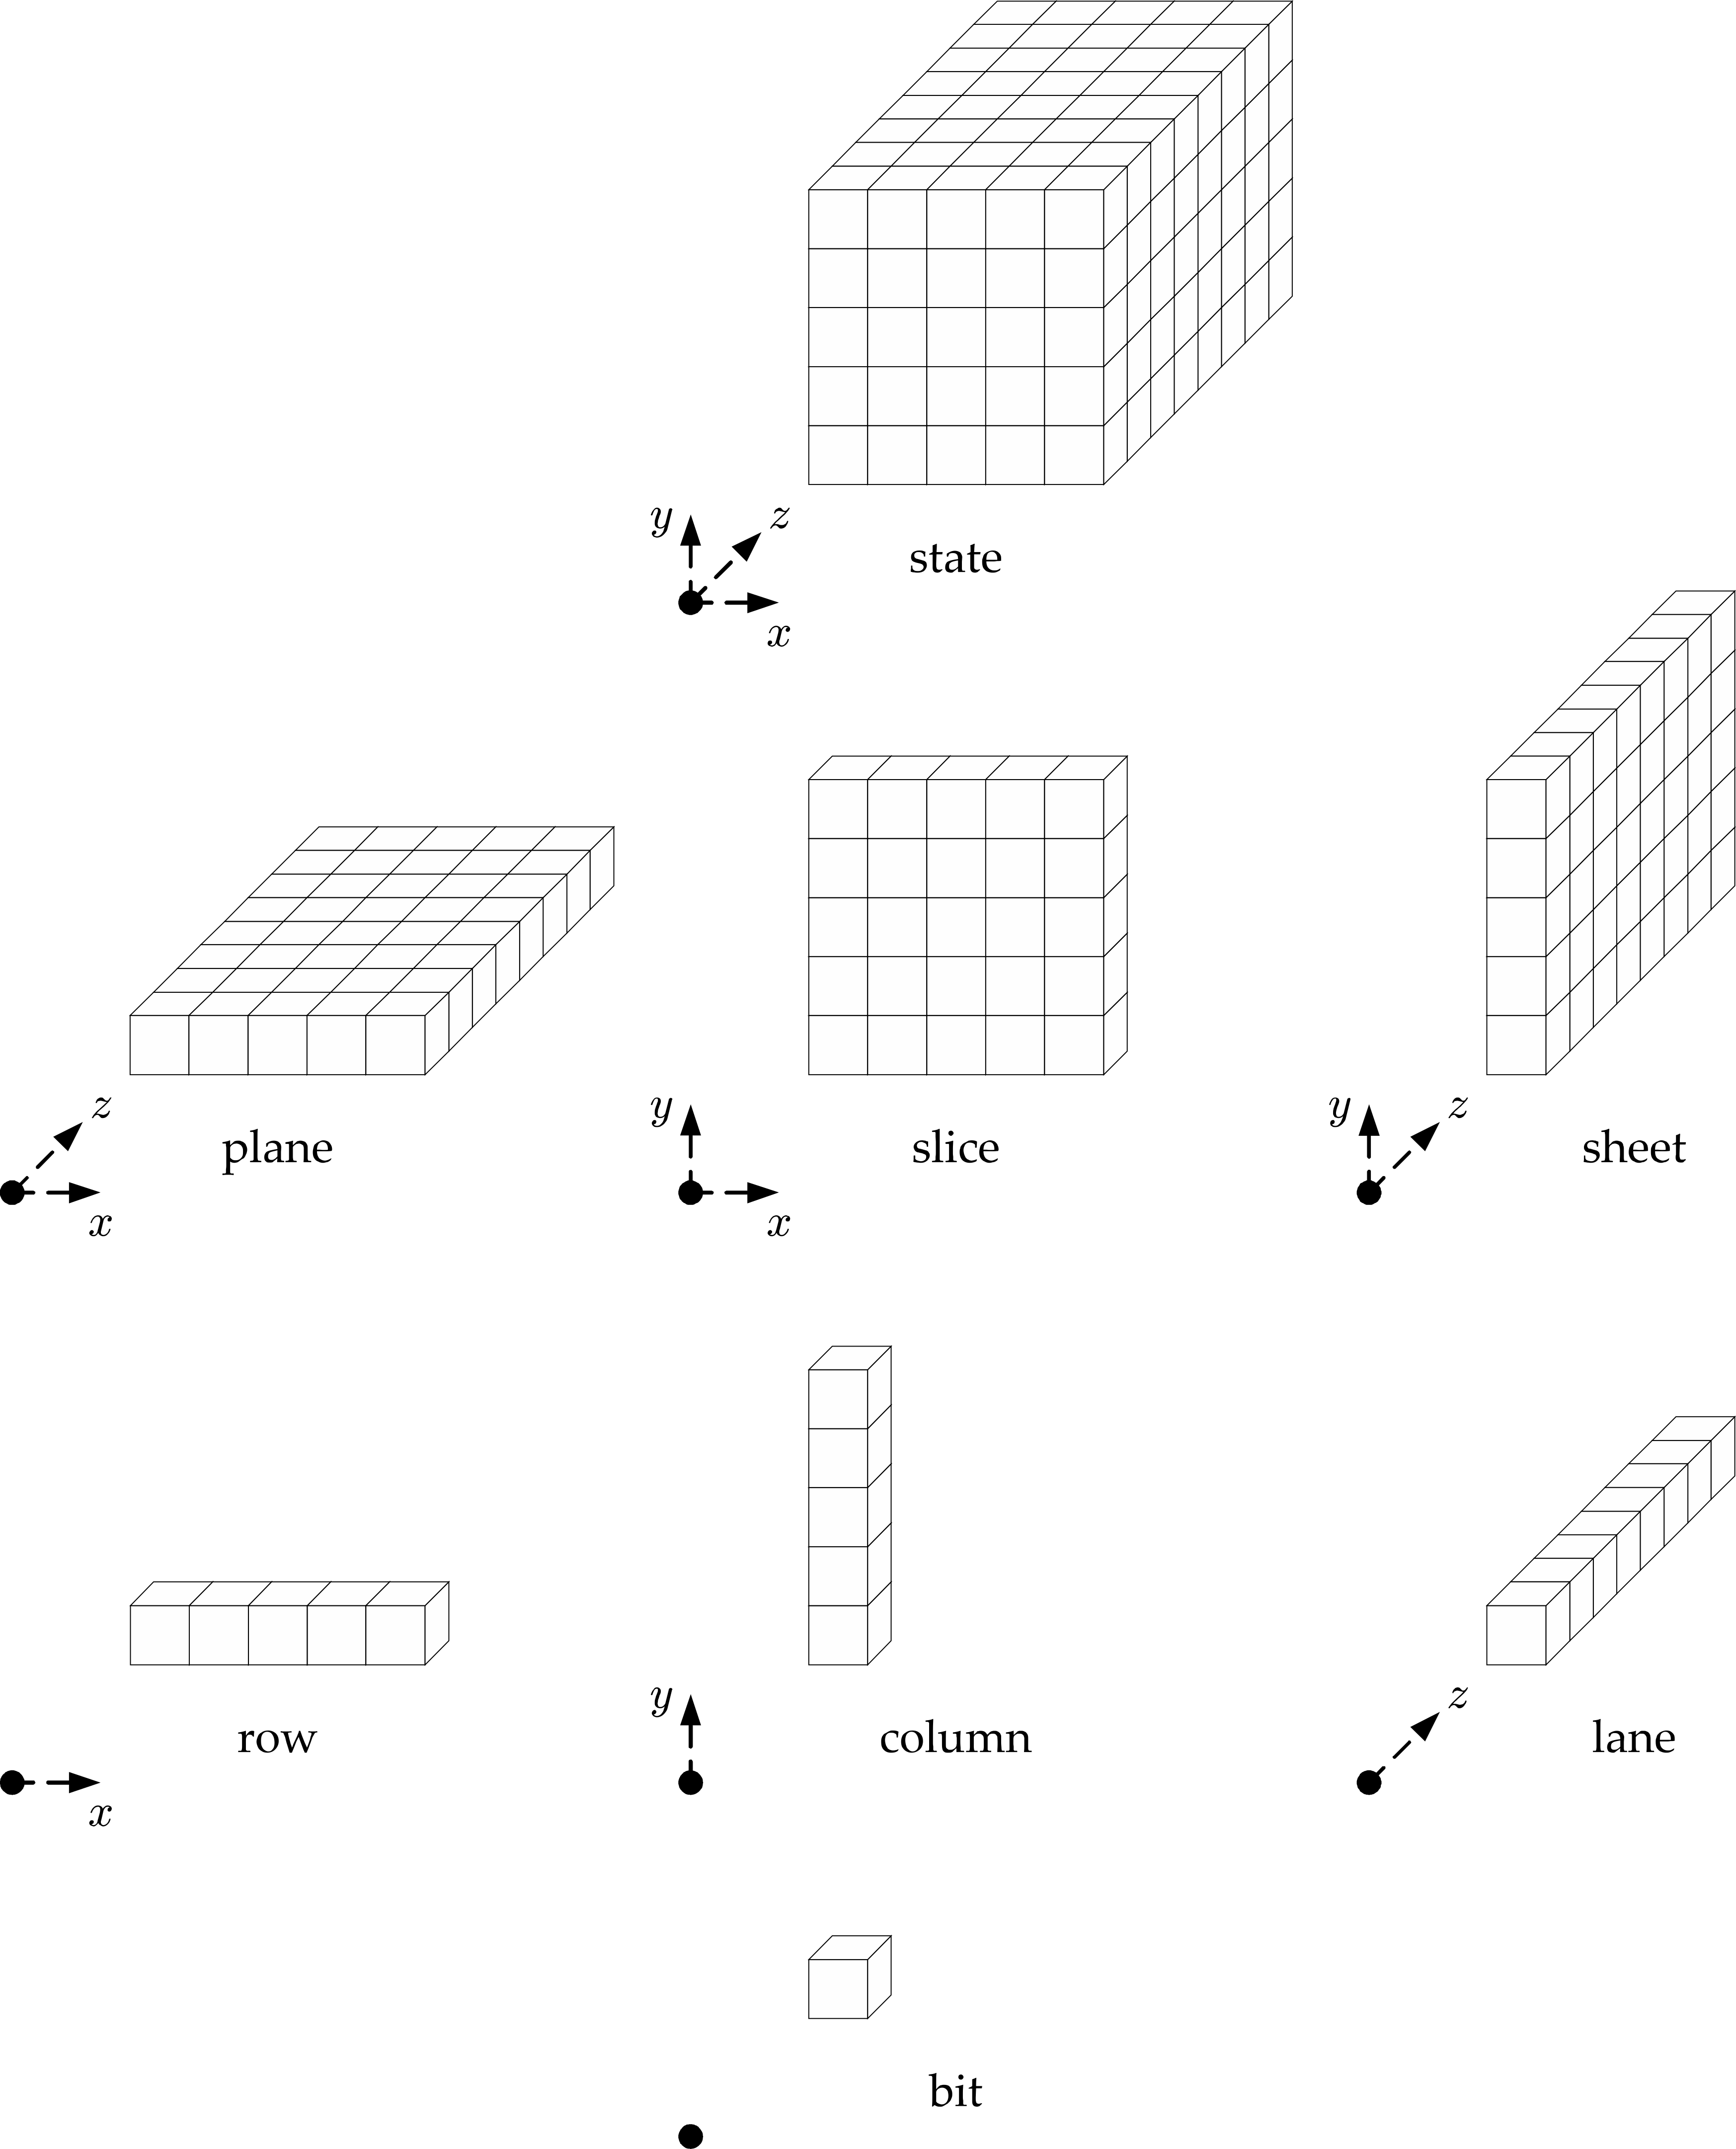
\includegraphics{images/keccak_state.png}
    \caption{notation for parts of the Keccak state array}
    \label{fig:keccak_state}
\end{figure}

The permutation is an iterated one, consisting of 24 rounds of $R$, where
\begin{equation*}
  R = \iota \circ \chi \circ \pi \circ \rho \circ \theta
\end{equation*}

is composed of five smaller phases:

$\begin{array}{rl}
  \theta:& C_{(x)} = \sum\limits_{y=0}^4 A_{(x,y)}\\
  &D_{(x)} = C_{(x-1)} + \text{rot}(C_{(x+1)},1)\\
  &A_{(x,y)} = A_{(x,y)} + D_{(x)}\\
  \pi \text{ and }\rho:& B_{(y,2x+3y)} = \text{rot}(A_{(x,y)}, r(x,y))\\
  \chi:& A_{(x,y)} = B_{(x,y)} + (B_{(x+1,y)} \times B_{(x+2,y)} + 1)\\
  \iota:& A_{(0,0)} = A_{(0,0)} + RC\\
\end{array}$\\

All operations are carried out in $GF(2)$, i.e. addition is bitwise XOR and
multiplication is bitwise AND. rot$(W,i)$ is a bitwise cyclic shift operation.
The constants $r(x,y)$ are rotation offsets. $RC$ is the round constant.
For more details, see~\cite{keccak_reference}.

%TODO: explain the phases properly


\section{Algebraic fault analysis}
Differential fault analysis (DFA) is an established technique for attacking
cryptographic algorithms, introduced over twenty years ago in~\cite{DFA_DES}.
It assumes that a fault has occured at a specific point in the execution of the
algorithm, and analyzes the propagation of a \emph{difference} between the
original state and the new, faulty state. It has been applied to many well-known
algorithms with great success, such as DES~\cite{DFA_DES}, AES~\cite{DFA_AES, DFA_AES_single-fault},
and the SHA-1 compression function~\cite{DFA_SHA-1_compression}. The direct
predecessor of the DFA attack was used to break RSA~\cite{boneh-demillo-lipton_RSA}.
SHA-3, likewise, has been shown to be vulnerable to fault injection with DFA,
first with single-bit faults~\cite{DFA_SHA-3_single-bit}, and later with byte
faults~\cite{luo2017relaxed}.

However, DFA can be very cumbersome, requiring complex and tedious analysis of
how the differential propagates through the algorithm. Even with an algorithm
such as Keccak, with algebraically simple internals, the differential propagation
is not exactly easy to follow.\footnotemark

\footnotetext{
    The reader is certainly invited to give it a try --- the byte-fault
    propagation in~\cite{luo2017relaxed} is quite bearable.
}

Algebraic fault analysis (AFA) sidesteps this problem. Instead of manually
analyzing the propagation, AFA uses an appropriately constrained SAT solver.
That is, it:
\begin{enumerate}
    \item encodes (part of) the cryptographic algorithm as Boolean statements
    \item encodes the fault model (assumptions about the fault: its position
          and effect) as Boolean statements
    \item gives the above to the SAT solver as constraints
    \item gives the (good output value, bad output value) pair to the SAT solver
          as constraints
    \item uses the SAT solver to do the work of calculating the implied secret
          bits
\end{enumerate}

SHA-3 is sucessfully attacked in~\cite{luo2018algebraic} using AFA, and the
attack is extended to an even more relaxed fault model (a 32-bit one) than
was possible with DFA, since AFA makes better use of the faulty outputs.

%TODO: a more detailed description of AFA on SHA-3 specifically is given in ...


\section{Implementation attacks and fault injection}
Cryptographic algorithms that are perfectly safe in theory can be successfully
attacked in practice by attacking not the algorithm itself, but its implementation.
Any implementation which exists in the real world is a perfect black box: it can
be observed and interacted with outside of its nominal inputs and outputs.

Implementation attacks can be roughly divided into passive and active ones.

Passive attacks, also called \emph{side-channel attacks} (SCAs), do not interfere
with the execution of the cryptographic algorithm, but observe the effects the
implementation has on its surroundings, which leak secret information.
There are many: power consumption, electromagnetic radiation, timing, even sound. % TODO: add references?
These (unintended) side effects can be thought of as transmitting secret
information over a noisy channel, hence the name.

Active attacks, on the other hand, interfere with the cryptographic algorithm
somehow. They rely on inducing faulty behaviour, e.g. skipping instructions or
flipping bits, hence the name \emph{fault attacks}. They inject faults into the
operation of the algorithm, so the practice is called fault injection.
The common ones are:
\begin{itemize}
  \item operating the device outside of its safe operating range
        (too high/low temperature or voltage, over- or underclocking the device)
  \item injecting transient voltage spikes in the supply voltage (a.k.a. $V_{cc}$ glitching)
  \item exposing the board to an electromagnetic field, of a sinusoidal wave (harmonic EMFI)
        or short pulses (pulsed EMFI)
\end{itemize}

%TODO: rewrite this ^ paragraph better

Since only pulsed EMFI is considered here, in the rest of the text EMFI refers
to pulsed EMFI.


\section{Genetic algorithms}\label{sec:GAs}
Evolutionary algorithms (EAs) are metaheuristic optimization algorithms,
inspired by biological evolutionary processes and phenomena such as mutation,
recombination, and natural selection.
In a way, they simulate the natural process of evolution: a solution
(i.e. point in the solution space) becomes an individual in the population.
These "individuals" are then valued using a \emph{fitness function}; better
solutions are fitter individuals, with a higher chance of surviving and procreating.
Thus the objective function (which we are optimizing) gets mapped to the fitness function
and, over a number of generations, the evolutionary process takes care of the optimization.

Every generation, a number of individuals are selected from the population to
reproduce, i.e. to become parents; fitter individuals are given preference.
Those individuals are in some way combined to produce offspring (new solutions).
There is a small chance of mutations in the offspring: this allows the introduction
of new elements to the solution, which otherwise may not have ever been generated
from the initial population by just selection and reproduction.

After generating the offspring, the population is (whole or in part) replaced
by the offspring: the next generation.

The outline of an evolutionary algorithm is given below:
\begin{algorithm}[h]\label{algo:evolutionary}
    \begin{algorithmic}
        \STATE $\mathit{population} \gets$ generate initial population
        \REPEAT
            \FOR{$\mathit{individua}l \in \mathit{population}$}
                \STATE evaluate fitness ($\mathit{individual}$)
            \ENDFOR
            \STATE $\mathit{parents}    \gets$ select ($\mathit{population}$)
            \STATE $\mathit{offspring}  \gets$ generate offspring ($\mathit{parents}$)
            \STATE $\mathit{population} \gets  \mathit{offspring}$

        \UNTIL{termination criterion met}

        \RETURN choose best individual ($population$)
    \end{algorithmic}
    \caption{evolutionary algorithm pseudocode}
\end{algorithm}

Mind that this is a fairly general outline.
The choice of selection and offspring generation makes all the difference.
Usually, however, offspring generation consists of two phases:
\begin{itemize}
    \item combining two (or more) parents to produce a child
    \item mutating the child with some probability $p$
\end{itemize}
It is not necessary for the entire population to be replaced in a generation.
A portion of the fittest individuals surviving across generations is called
\emph{elitism}; this could also be regarded as "cloning" the old solutions into
the next generation, so it fits in the outline given above.

This three-phase algorithm, when we represent the solution as a string of numbers,
is called a \emph{genetic algorithm} (GA).
In analogy to real life (though not exactly the same), this representation is
called the \emph{chromosome} (or \emph{genotype} or \emph{individual}; they're
interchangeable); multiple chromosomes are combined using \emph{crossover}
(or \emph{recombination}) to produce offspring.

However, what exactly falls under genetic algorithms and the exact lines between
GAs and other evolutionary algorithms can at times be a bit vague. That's okay,
since it's a metaheuristic we're talking about.
To instance this \emph{metaheuristic} into a \emph{heuristic}, we need to replace
these somewhat vague terms (selection, crossover, mutation, genetic representation)
with concrete ones. This is left up to the implementer.



\chapter{Fault injection}\label{ch:fault_injection}
One obvious prerequisite for doing fault injection is a physical device running
an actual algorithm to inject faults in. A cryptographic algorithm can be found
easily; a susceptible one, with a bit of literature review. A device to
attack, as well as the necessary equipment for glitching it, can be a bit harder
to find.

This chapter is laid out thus: section \ref{sec:definitions} introduces the
definitions used in the rest of the paper; section \ref{sec:setup} covers
the physical setup used for the experiments; section \ref{sec:parameters}
presents the parameters used, and section \ref{sec:search_space} the big
motivation for having a search at all. Sections \ref{sec:assumptions} and
\ref{sec:objectives} take care of the implicit assumptions on the search
space and our requirements for the algorithm; section \ref{sec:note_on_algorithms}
covers the impact the underlying cryptographic algorithm on the parameter
space; last, section \ref{sec:practical_considerations} covers some practical
implications of EM fault injection for the algorithm.



\section{Definitions}\label{sec:definitions}
When discussing the search and possible outputs of the algorithm,
\begin{description}
    \item[a point] is a distinct set of parameters, i.e. a point in the parameter space.
    \item[a measurement] is the result of a single attempt at glitching the target with those parameters.
\end{description}

A single point may measured be measured multiple times, since trying the same
parameters multiple times does not necessarily always yield the same response.
In the rest of this thesis, only single-measurement and five-measurement points
are used.

When counting the faulty measurements (i.e. those resulting in a faulty
response), we distinguish between:
\begin{enumerate}
    \item the total number of faulty measurements,
    \item the number of distinct faulty responses (i.e. ``unique faulty measurements'').
\end{enumerate}

The difference is that if a measurement results in a before-seen faulty output,
the second one will not be counted this second time around.
To better illustrate this: say we find a set of parameters $S_1$, which is
measured five times, with one of the measurements giving a faulty output $h_1$.
Later, we find some other set of parameters $S_2$ that results in two faulty
outputs, $h_1$ and $h_2$. Out of the ten measurements performed in total, three
of these are considered faulty, but with only two distinct faulty responses:
$h_1$ and $h_2$, since $h_1$ is not counted twice.
For the purposes of exploitation, the number of distinct faulty responses is
more interesting.

We classify the board response in one of the following classes:
\begin{description}
    \item[NORMAL]   -- for normal behaviour, meaning the board performs as if it wasn't glitched
    \item[RESET]    -- the board did not reply at all, requiring a reset to restore to normal operation
    \item[SUCCESS]  -- the board produces an output/ciphertext/signature/hash different than the correct one
    \item[CHANGING] -- for each point, 5 measurements are performed. If all measurements are in the
                       same class, the point is put into one of the first three classes; otherwise
                       it goes into the CHANGING class.
\end{description}

\emph{Random search} refers to just randomly choosing points to scan.
\emph{Grid search} is scanning points in a regularly-spaced grid that covers all
or part of the search space.
For the purposes of this thesis, random search is the baseline search algorithm.


\section{Experimental Setup}\label{sec:setup}
For the target, a Cortex-M4 STM32F407IG (Riscure ``Pi\~{n}ata'') board was used,
running a C implementation of SHA-3. This implementation was taken from the WolfSSL
library~\cite{WolfSSL}, so as to have a real-world algorithm instead of a toy one.
The board communicates to a PC by a serial interface and is powered by an external
power supply (\SI{3.3}{\volt} DC). For inducing an electromagnetic pulse, the
Riscure EM probe is used, as well as their VCGlitcher device that controls it.
The board and the EM probe are set up on an XYZ table which moves the probe
around in space. The whole setup is controlled by code written in Python; for
communicating with the Riscure equipment, Python bindings for the VCGlitcher
C API are used.\footnotemark

\footnotetext{
   Currently, due to the provided DLL being a 32-bit one, a 32-bit Python
   interpreter is required. This may change in the future.
}

Besides the serial interface, the board has a number of I/O pins which it can
toggle to high or low; the only one here used is the "trigger" pin. This pin is
used to signal to the VCGlitcher device that the cryptographic operation is in
progress; this is used as a reference point for injecting the fault. While this
slightly detracts from the realism of the attack, it greatly simplifies testing.
(It does not make much difference for the vulnerability status of the device,
since in real life the attacker only needs to spend more time figuring out the
timing.)

In the case that the board gets stuck in an illegal state after a glitch, it
needs to be reset. The only reliable way to reset this particular board is by
cutting its power, which can take a significant fraction of a second, depending
on the capacitors. A pause of \SI{100}{\milli\second} was used for this.

The physical dimensions of the chip package are $24 \times 24$\,\si{\milli\metre}
Repositioning error of the XYZ table is \SI{0.05}{\milli\metre}, which gives
a spatial grid of at most $480 \times 480$. However, the limiting factor here
is most likely the size of the probe tip (and its internal coil), which is much
larger.

%(TODO: compare to other people's more precise probe tips?)
All of these will, of course, vary depending on the chip and the equipment at
hand; even for different variants of the Piñata, the capacitors differ.
A more precise XYZ table, a smaller probe (such as in e.g.~\cite{precise_probe_tips}),
or a smaller chip will give different spatial resolutions.


\section{Parameters}\label{sec:parameters}
There are multiple parameters to vary to affect the probability of causing a
fault: position of the probe tip (X, Y, and Z), pulse intensity, time offset
of the pulse, pulse duration, shape and angle of the probe tip, and pulse shape.

In the experiments conducted, only a subset of these are considered:
\begin{description}
  \item[position] -- two parameters (X and Y), since the distance from the board
        (Z) can be compensated by a change in intensity. The $(x,y,z)$ position
        in real space is mapped by the interfacing code to an $(x,y)$ position
        in the unit square $[0,1]^2 \in \mathbb{R}$.
  \item[glitch intensity] -- regulates the voltage of the pulse. The SDK manual
        suggests that it is a percentage of power used~\cite{RiscureVCGmanual},
        so it makes sense to map it to real values in $[0,1]$.
  \item[time offset] -- between 367 and 375\,\si{\micro\second}, because that is
        where the injection point must be, for the code we are running. The offset
        is encoded as an integer value (number of \SI{2}{\nano\second} ticks).
  \item[number of repetitions of the pulse] -- a primitive form of pulse shape.
        This parameter is set to be in the (obviously, integral) range $[1, 10]$.
\end{description}

The pulse duration stays constant at a fixed value of \SI{40}{\nano\second}.
Similarly, the shape and angle of the probe tip is not varied, since changing
those cannot be easily automated.

Most parameters are within $[0,1]$, but we can map the other ones to that
interval as well, by taking its "percentage": a parameter with range $[A,B]$,
a value $x \in [A,B]$ is mapped to $y = \frac{x-A}{A-B}$, which is in $[0,1]$.
With everything mapped to $[0,1]^5$, we can now define any length or distance
to be the standard Euclidean distance in this image of the parameter space.


\section{Search Space Size}\label{sec:search_space}
One might wonder: why use a heuristic at all? What's wrong with a "dumb"
approach to parameter optimization? Let's consider the straightforward
approach: an exhaustive search.

The maximal spatial resolution, as I mentioned above, is $480 \times 480$ for
this particular setup; a better setup would have an even higher one. For the
time offset, the resolution is \SI{2}{\nano\second}; for a reasonable range,
I'll put the interval between 367 and 375 microseconds, since this was measured
as the interval containing the fault injection point -- this gives us a total of
4\,000 different values; for the glitch intensity, there's really no good rule
for determining the smallest meaningful increment, but a 1\% increment seems
a fairly reasonable (if conservative) estimate based on visual estimates of
the results, which would give a range of 100 values; the repetitions parameter
in range $[1,10]$ gives an extra 10 values.

The total size is therefore $480*480*4\,000*100*10\approx 10^{12}$.
At $\approx0.16$ seconds per measurement, and five measurements per point, this
results in 29\,203 years to conduct an exhaustive search. Even if completely
ignoring everything but X, Y, and offset, an exhaustive search would still
take 29.2 years to finish.



\section{Some assumptions on the search space}\label{sec:assumptions}
From the viewpoint of the optimization algorithm, the device should be as close
as possible to a black box. That is to say, the algorithm should not have built-in
assumptions that would be broken by running it for another device or cryptographic
algorithm. However, I do make some assumptions:
the objective function is not a golf-course. In a golf-course function, the
gradient in the fitness landscape doesn't lead to optimal solutions, which tend
to "pop out of nowhere", all of a sudden. Given the nature of EM glitching, the
transition between different kinds of behaviour should be reasonably gentle; the
reasoning behind it is that a very weak EM pulse will not affect the target at all,
and we will observe normal behaviour. Conversely, a very strong EM pulse will
completely dishevel its operation and even potentially damage it. Consequently,
we should expect faulty behaviour to occur somewhere between those two extremes,
i.e. along the class border; in other words, there are blobs of RESETs in a sea
of NORMALs, wrapped in a thin layer of SUCCESSes and CHANGINGs.

Additionally, offset ranges (min. to max. offset) are set by the user,
based on a rough expectation of the duration of the cryptographic algorithm.



\section{A note on underlying algorithms}\label{sec:note_on_algorithms}
Some of the early scans and tests were done not on the Piñata running SHA3-512,
but Piñata running EdDSA (also taken from WolfSSL). There exists a difference
between their respective search spaces: the parameters and the parameter ranges
are largely the same (there is a difference in the offset range, since EdDSA
takes $\approx$\SI{30}{\milli\second} to run, SHA3-512 only $\approx$\SI{0.4}{\milli\second}),
but underlying calculation and the "look" of the parameter space is different.
In EdDSA, the vast majority of the time is spent performing a scalar
multiplication on the Ed25519 curve, and the parameter space has one big
blob of RESETs, the rest being filled by NORMALs. For SHA3-512, all the
time is spent on the Keccak-$f$ transformation, and the parameter space
has not only the (substantially smaller) blob of RESETs, but also several
blobs composed of mostly CHANGING points, with a number of RESETs and SUCCESSes.
Figure \ref{fig:parameter_spaces} shows what the parameter space looks like
for both of these.

CHANGING points (and some other features) were not present from the start;
they were implemented just before switching to SHA-3, hence most scans on EdDSA
don't have them, and use single-measurement points instead. The process of
selecting the algorithm and its hyperparameters was not a systematic one
with extensive tuning, but a pragmatic one of choosing the most promising
options within the timeframe.

\begin{figure}[htbp]
    \centering
    \begin{subfigure}[b]{0.48\textwidth}
        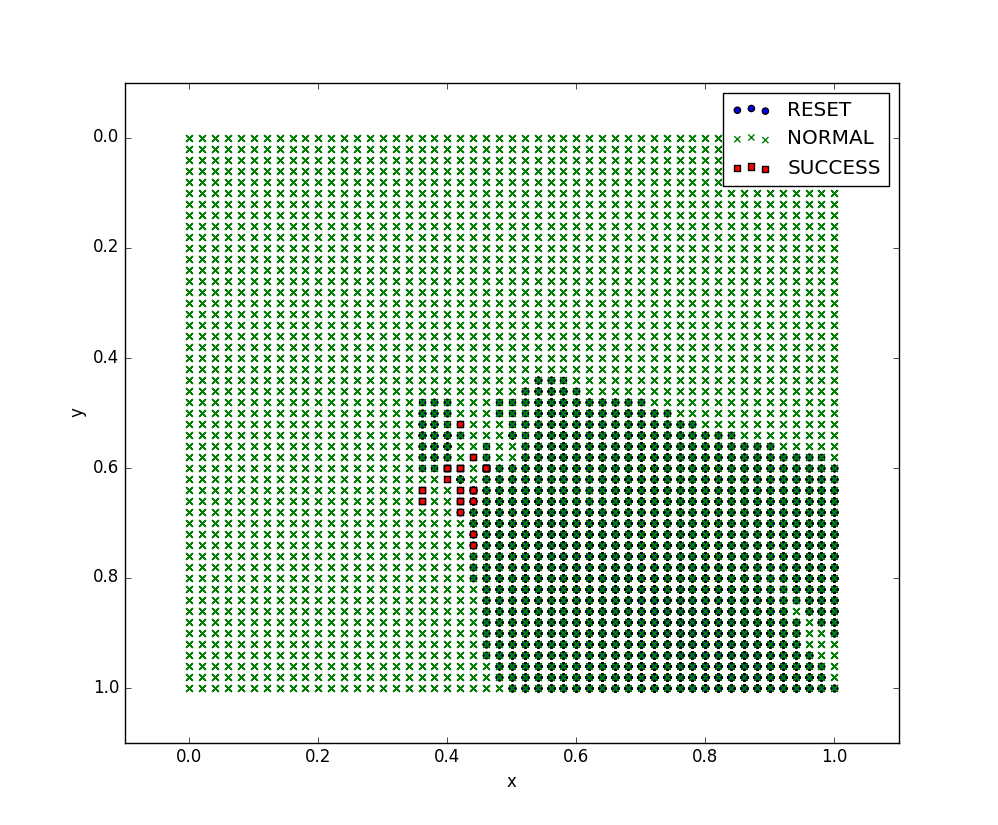
\includegraphics[width=0.95\linewidth]{images/plots/EdDSA_space_all_2D.png}
        \caption{EdDSA, in the 2 spatial dimensions}
    \end{subfigure}
    \hspace{8pt}
    \begin{subfigure}[b]{0.48\textwidth}
        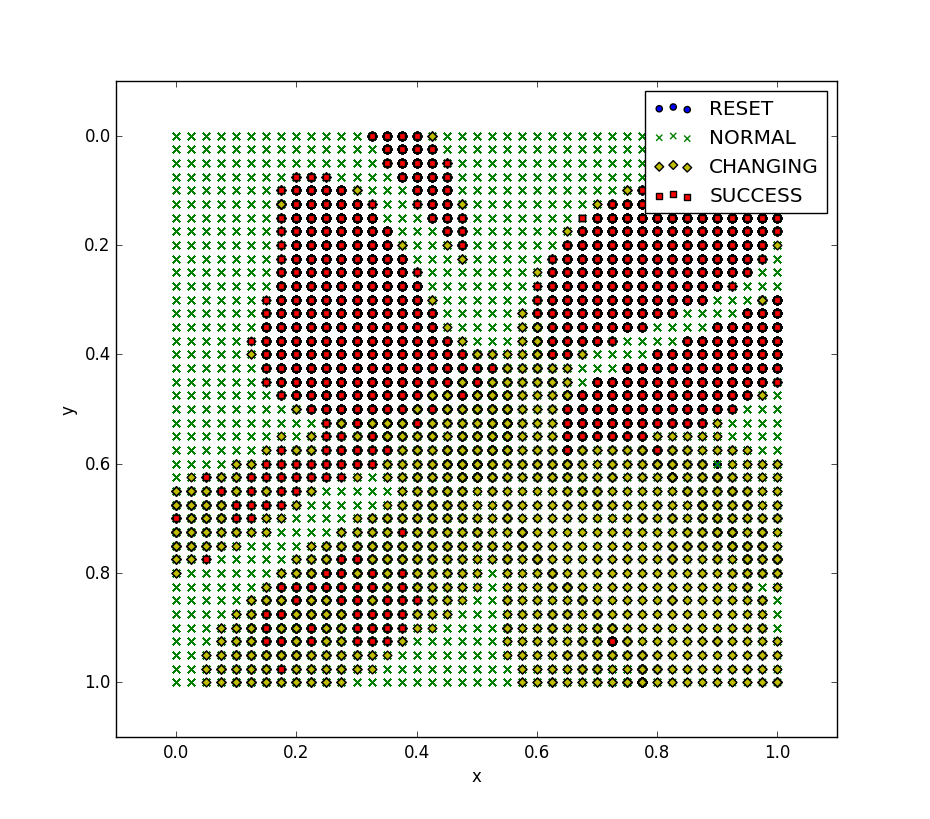
\includegraphics[width=0.95\linewidth]{images/plots/Keccak_space_all_2D.png}
        \caption{SHA3-512, in the 2 spatial dimensions}
    \end{subfigure}

    \begin{subfigure}[b]{0.48\textwidth}
        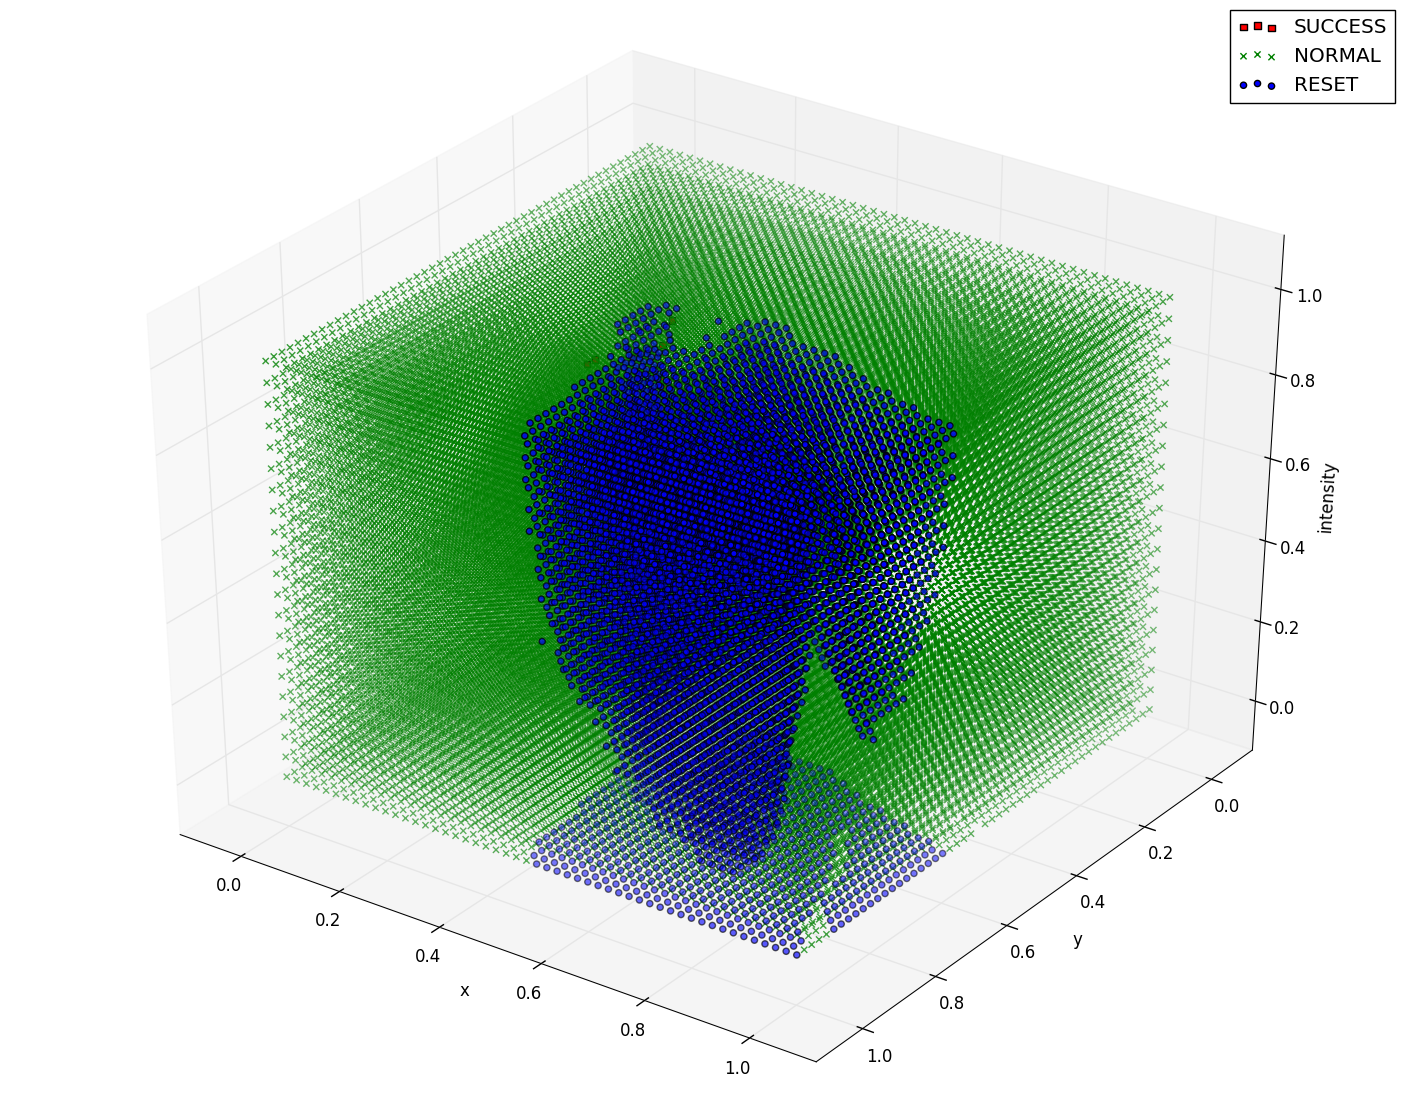
\includegraphics[width=0.95\linewidth]{images/plots/EdDSA_space_all_3D.png}
        \caption{EdDSA, 2 spatial dimensions and intensity}
    \end{subfigure}
    \hspace{8pt}
    \begin{subfigure}[b]{0.48\textwidth}
        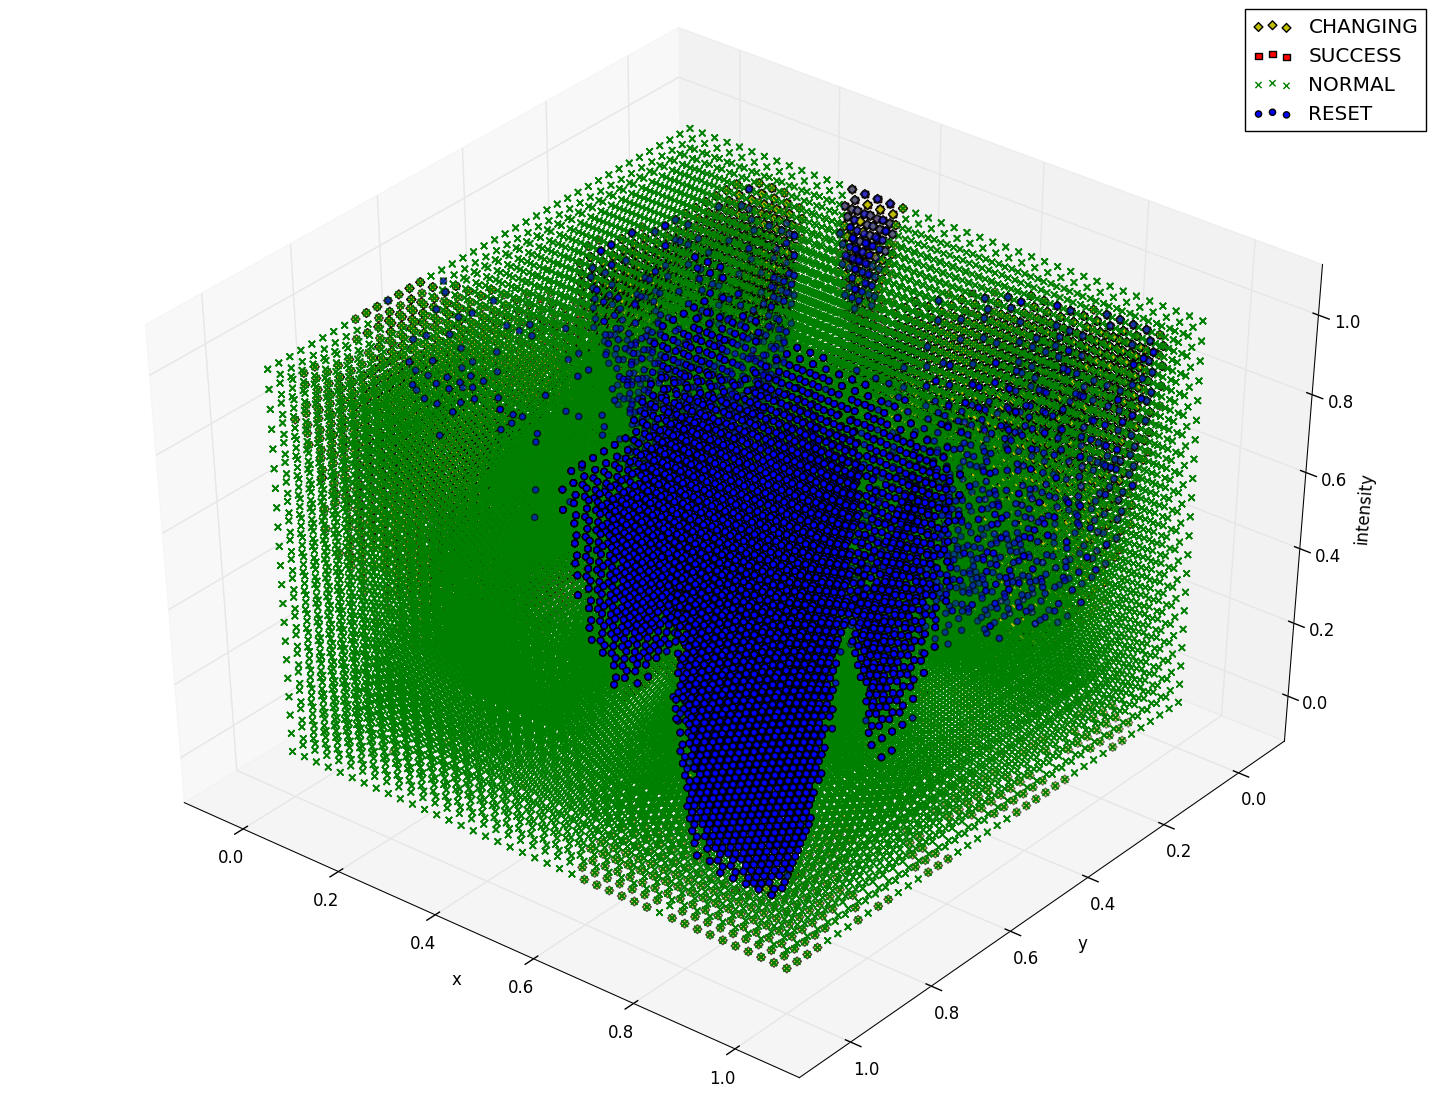
\includegraphics[width=0.95\linewidth]{images/plots/Keccak_space_all_3D.png}
        \caption{SHA3-512, 2 spatial dimensions and intensity}
    \end{subfigure}

    \begin{subfigure}[b]{0.48\textwidth}
        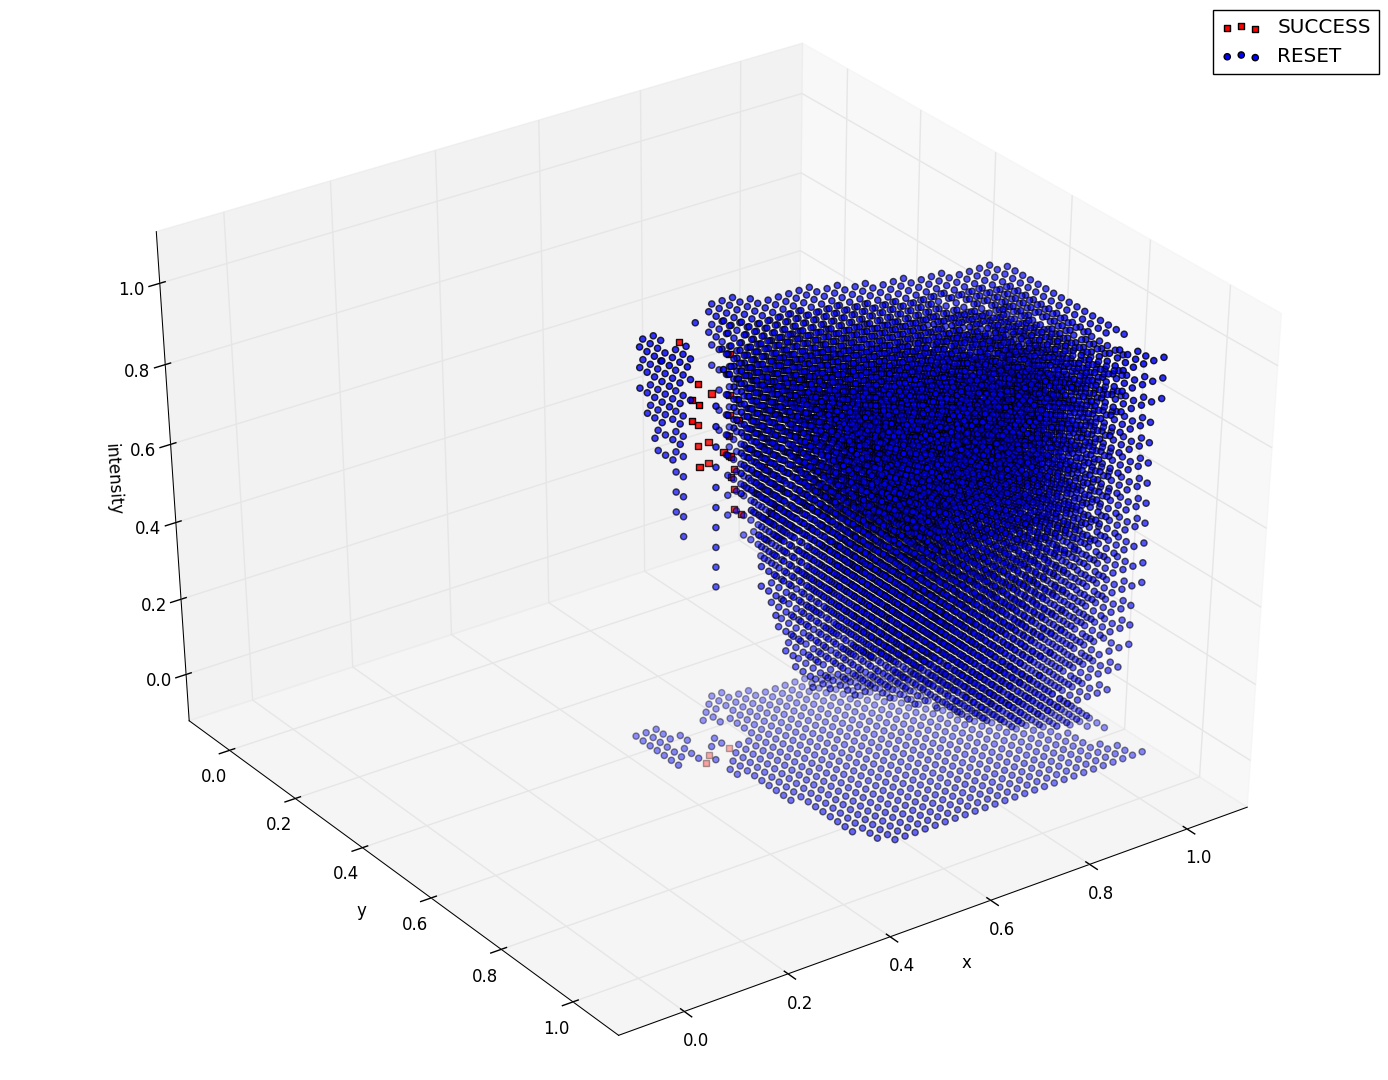
\includegraphics[width=0.95\linewidth]{images/plots/EdDSA_space_nonormal_3D.png}
        \caption{EdDSA, but without NORMAL points for clarity}
    \end{subfigure}
    \hspace{8pt}
    \begin{subfigure}[b]{0.48\textwidth}
        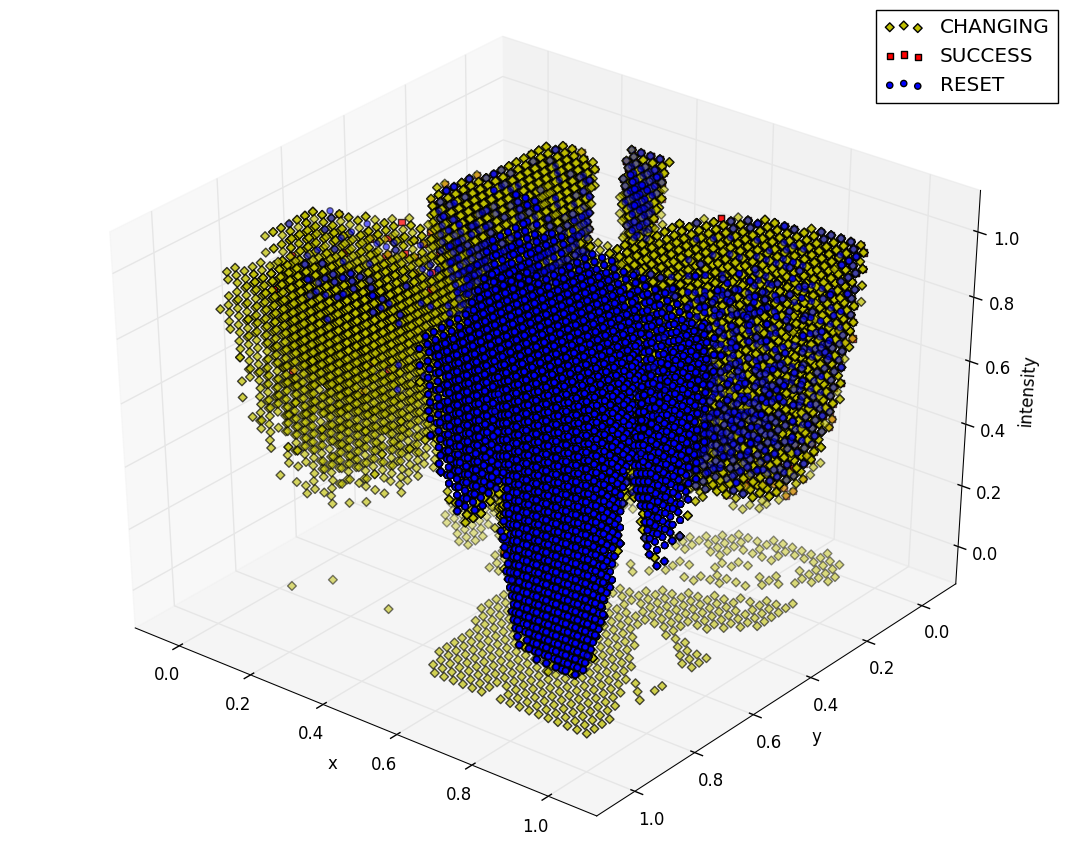
\includegraphics[width=0.95\linewidth]{images/plots/Keccak_space_nonormal_3D.png}
        \caption{SHA3-512, but without NORMAL points for clarity}
    \end{subfigure}

    \caption{parameter space visualization, for EdDSA and SHA3-512}
    \label{fig:parameter_spaces}
\end{figure}



%More in detail, our algorithm consists of two separate phases as follows:
%\begin{enumerate}
%    \item The first phase is a genetic algorithm where we run it for  20 generations with population size 50.
%    \item Only when the genetic algorithm is done, we start with the local search, which takes 10 randomly chosen points in neighbourhood of each SUCCESS point. Note that this is a significant difference from related works where both GA and local search worked at the same time. We opted first to concentrate on exploration aspect -- GA (to explore various regions of the target) and only after that on exploitability aspect -- local search (to concentrate on more promising regions). Naturally, GA itself has also exploitability component that is especially manifested in the crossover operator but we also designed a custom made crossover operator that promotes exploration perspective.
%\end{enumerate}


\section{Objectives}\label{sec:objectives}
The requirements for this optimization algorithm are:
\begin{description}
    \item[Good coverage of the parameter space] -- since we do not know where the
          exploitable faults are located, we need to explore the search space efficiently.
    \item[Speed] -- we require the algorithm to be fast in finding the faults, otherwise
          there is no advantage of using it when compared to the baseline.
\end{description}

These two requirements somewhat conflict with each other. Because most of the
parameter space is useless (i.e. has no faults), covering enough space to be
reasonably secure we did not miss anything important means potentially wasting
a lot of measurements.

Usually, the objective function guides the optimization algorithm towards better
solutions, and the algorithm ends when it finds what it considers to be the best
one. Here, we don't want just a single "best" solution since not every fault
that's found will also be exploitable, and there are situations where more than
one are required; instead the aim is to obtain multiple good solutions.



\section{Practical Considerations}\label{sec:practical_considerations}
Commonly, optimization algorithms (and nature-inspired metaheuristics in
particular) rely on a large number of iterations. Another assumption usually
made is that the evaluation of possible solution points is uniform. Here,
however, we have expensive measurements, where the cost of evaluation depends
not only on the properties of the point itself, but also the context of its
evaluation.
%Although our algorithm consists of genetic algorithm and local search, we denote
%it often as genetic algorithm but we always consider it to have also local search
%phase. We do not call our technique a memetic algorithm since the GA and local
%search phases are separated.
%
When considering EM fault injection, the probe tip has to physically move to
a different point. To do this with sufficient precision requires a non-negligible
amount of time -- the exact amount varies depending on the setup, but it can be
up to several seconds per measurement. In comparison, a reset requires just a
fraction of a second (for this board, $\approx$\SI{100}{\milli\second} to do it
reliably). The measurement part itself is even faster -- \SI{30}{\milli\second}
or less. Thus, the order in which points are evaluated matters.

Even with an optimal routing for any batch of $N$ points, splitting the
evaluation into more batches means more time wasted. For population-based
algorithms, this translates to small population sizes being less efficient
than large ones. Additionally, we may want to get a glimpse of the results
even before the scan is finished, especially for long-running scans. In the
case of a random or grid scan, this requires splitting the scan into batches
where each covers more or less the whole parameter space, since scanning points
in the optimal (or nearly-optimal) order results in uneven coverage: as a
general rule, a segment the shortest Hamiltonian path from any given starting
point will not evenly cover the XY-plane, but instead a small part of it.

%TODO: calculate exactly how much less efficient?




\chapter{Optimization}\label{ch:optimization}
Now, to deal with the optimization itself.

Since EM fault injection is an \emph{expensive} optimization problem, I created
an emulator of the board to respond in its stead. While most scans were in the
end done on the actual Piñata board, the emulator helps to predict and visualize
behaviour of different algorithms (or the same algorithm, but differently
parametrized) over multiple runs, with only a fraction of the runtime cost.
However, we can only expect this if the behaviour of the emulator closely
matches that of the board. This poses a problem: how do we achieve this?
Obviously, without modeling the chip itself (which would be a large problem
in and of itself), the emulator must rely on samples of the objective function.

The straightforward solution would be to exhaustively sample the parameter space
and use a lookup table, but as mentioned in section \ref{sec:search_space}, it's
impossible in terms of time, and very hard in terms of space ($\approx 5 \cdot
10^{12}$ measurements!). What \emph{is} possible, however, is a lower-resolution
grid scan, with interpolation between points. This was, in fact, performed: the
largest of these is a grid scan with $1/40$ resolution in the XY-plane, $1/20$
resolution in the intensity dimension, 9 offset values (from \SI{367}{\micro\second}
to \SI{375}{\micro\second}, with \SI{1}{\micro\second} step), and with repetitions
set to 1. This gives $41 \times 41 \times 21 \times 9 = 317709$ points; with an
average of \SI{1.125}{\second} per point, this takes around 100 hours, or a bit
over four days. Given that this is a grid scan, it greatly simplifies storage
and nearest-neighbour lookup: caching it as a bare NumPy array in a binary file
takes up less than \SI{3}{\mebi\byte} of space, the loading takes just a
fraction of a second, and once in RAM, the lookup is as trivial as it gets.
This is relatively easy to extend to $k$-nearest neighbours.

Another variant, made convenient by the availability of a number of scans of the
parameter space, would be to abandon the notion of a regular grid, aggregate all
those scans, and use that as the underlying information.

%TODO: more information on this?

In any case, the emulator will be intrinsically limited due to being bound to
actual data.




\section{Simple GA}
First, a simple genetic algorithm was tried out, with a single elite individual.
The initial population is generated by sampling uniformly at random within the
parameter ranges.

\subsection{Selection and crossover}
Several selection algorithms were used: roulette-wheel selection, 3-tournament
selection, and a variation on roulette-wheel selection with class awareness.
This last one was inspired by the work in~\cite{GlitchItIfYouCan}; its
pseudocode is given below:
\begin{algorithm}
    \small
    \begin{algorithmic}
    \STATE $N \gets \text{length}(population)$
    \STATE $elite\ size \gets 1$
    \STATE $population_{new} \gets \varnothing$
    \FOR {i in range($N - elite\ size$)}
        \STATE $parent_1  \gets$ random choice ($population$)
        \IF { there exist individuals $\notin$ class ($parent_1$)}
            \STATE $parent_2 \gets$ random choice (other classes)
        \ELSE
            \STATE $parent_2$ $\gets$ random choice ($population \setminus \{parent_1\}$)
        \ENDIF
        \STATE $child \gets$ classaware crossover ($parent_1$, $parent_2$)
        \STATE $child \gets$ mutate ($child$)
        \STATE $population_{new} \gets population_{new} \cup \{child\} $
    \ENDFOR
    \end{algorithmic}
    \caption{pseudocode for the class-aware roulette-wheel selection}
\end{algorithm}

The class-aware crossover here simply returns a point halfway between the parents,
if the parents are from different classes; otherwise it acts as a normal crossover.
The idea behind this is simple: after finding a RESET, use it to locate the class
border area, and concentrate there.

Of the selections, roulette-wheel selection was chosen for further testing.
As it turns out, the class-aware selection did find a part of the class border
area very fast, and converge there; however this was only a very small part of
the border, and the algorithm is not able to "recover" from this convergence,
but it will instead stay on the same small area, nor mapping out the rest of
the space.
3-tournament selection was not chosen, since it appeared to be too aggressive,
i.e. it exerted overly high selection pressure for the problem at hand.
It works by randomly choosing individuals three at a time, in "tournaments".
The lowest-ranking of the three is discarded, and the other two are used as
parents. The tournaments are held until enough children have been produced.


The "normal" crossover, however, is not a standard GA crossover, but different.
Its pseudocode is given below in Algorithm \ref{algo:custom_crossover}.

\begin{algorithm}
    \small
    \begin{algorithmic}
        \STATE \textbf{Input:} $parent_1, parent_2$, two chromosomes, each a list of FI parameters
        \STATE \textbf{Output:} $child$, the resulting child
        \FOR {each parameter $p$ in range($N - elite\ size$)}
            \STATE $child.p \gets $ random value in interval $[parent_1.p, parent_2.p]$)
        \ENDFOR
        \RETURN $child$
    \end{algorithmic}
    \caption{pseudocode for custom GA crossover}
    \label{algo:custom_crossover}
\end{algorithm}

For comparison, the standard single-cut crossover is given as Algorithm
\ref{algo:standard_crossover}; the uniform crossover is not much different.
In terms of behaviour, it would be best to consider the geometric interpretation.
A vector of $k$ parameters can be viewed as a point in $k$-dimensional space.
Two such points -- the parents -- define an axis-aligned $k$-dimensional hypercube.
The "normal" crossover calculates the child as a random point from within
that hypercube; the standard crossovers, in contrast, calculate the child as
one of the corners of the hypercube. If the child has $l$ parameters of parent$_1$,
it will be at a Hamming\footnotemark distance of $k-l$ from parent$_1$, and $l$
from parent$_2$.

\footnotetext{
    \emph{Hamming distance} might not be the technically correct term here,
    but it is easy to see the 1-to-1 correspondence between the edges of \emph{this}
    $k$-dimensional hypercube and the set $\{0,1\}^k$ of length-$k$ bitstrings:
    strings are corners, edges are bitflips.
}


\begin{algorithm}
    \small
    \begin{algorithmic}
        \STATE \textbf{Input:} $parent_1, parent_2$, two chromosomes, each a list of FI parameters
        \STATE \textbf{Output:} $child$, the resulting child
        \FOR {each parameter $p$ in range($N - elite\ size$)}
            \STATE $child.p \gets $ random choice ($parent_1.p$, $parent_2.p$)
        \ENDFOR
        \RETURN $child$
    \end{algorithmic}
    \caption{pseudocode for standard GA crossover}
    \label{algo:standard_crossover}
\end{algorithm}


\subsection{Mutation}
As for the mutation, its task is to ensure adequate exploration of the search
space. Its exact form shouldn't make a great difference for the successfulness
of the algorithm, as long as the final algorithm doesn't have any "blind spots",
i.e. it doesn't leave some parts of the search space unreachable by the algorithm.
The pseudocode of the mutation I used for this algorithm is given in Algorithm \ref{algo:mutation}.

\begin{algorithm}[!htbp]
    \small
    \begin{algorithmic}
        \STATE \textbf{Input:} $p_{MUT}$, the mutation probability
        \STATE \textbf{\hphantom{Input:}} $Q$, an upper limit on the step size
        \STATE \textbf{\hphantom{Input:}} $individual$, a solution to mutate
        \STATE \textbf{Output:} $individual'$, the mutant
        \STATE $individual' \gets \text{copy}(individual)$
        \FOR {each parameter $P$ except repetitions}
            \STATE with probability $p$:
            \STATE ~~~~$individual'.P \gets $ $individual.P + $ random choice from interval $[-\frac{Q}{2}, \frac{Q}{2}]$
            \STATE clip value of $individual'.P$ to within allowed range
        \ENDFOR
        \STATE with probability $p$:
        \STATE ~~~~$individual'.repetitions \gets $ random integer from the allowed range
    \end{algorithmic}
    \caption{pseudocode for mutation}
    \label{algo:mutation}
\end{algorithm}


Its per-parameter nature increases the probability that at least \emph{some}
mutation will happen. It also means that significant jumps will tend to be mostly
axis-aligned. The effect is somewhat similar to having a traditional crossover:
many points on perpendicular lines, seemingly radiating from a hotspot; however
the effect is weaker than with a single-cut crossover and a standard mutation
which twiddles all the parameters at once. See figure \ref{fig:weaker_effect}
for a picture of this.

\begin{figure*}[htp]
    \vspace{-50pt}      % so the bottom caption doesn't cover the page number
    \centering
    \begin{subfigure}[b]{\textwidth}
        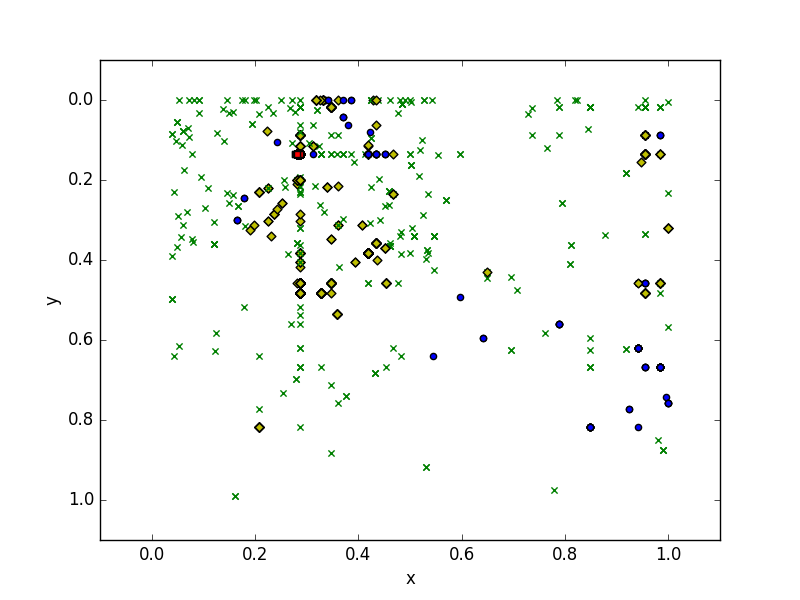
\includegraphics[width=\textwidth]{images/mutation_crossover_effect_comparison_traditional.png}
        \caption{single-cut crossover with a standard all-parameters-simultaneously mutation}
    \end{subfigure}

    \begin{subfigure}[b]{\textwidth}
        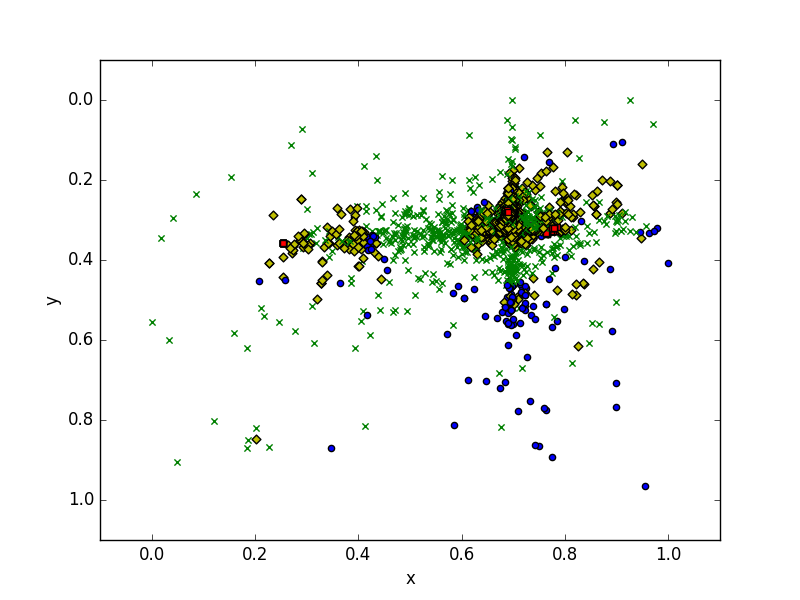
\includegraphics[width=\textwidth]{images/mutation_crossover_effect_comparison_myalgo.png}
        \caption{the custom within-hypercube crossover with a per-parameter mutation}
    \end{subfigure}
    \caption{A comparison of the effects of a per-parameter mutation with custom
             crossover vs. all-parameter mutation with single-cut crossover. Both
             runs have 50 generations of 50 units each, and use the same $p_{MUT}$.
    }
    \label{fig:weaker_effect}
\end{figure*}


\subsection{Fitness function}
Fitness values are set according to the class: SUCCESS has the highest fitness
(10), followed by CHANGING (variable), then RESET (5), and finally, NORMAL (2).
CHANGING points' fitness depends on its underlying measurements: a mix of NORMAL
and RESET points is somewhat better than all measurements being RESET or NORMAL
points, and adding SUCCESSful individual measurements into the mix moves the
fitness close to an all-SUCCESS point. With these requirements in mind, the
following formula was chosen for the fitness of a CHANGING point:
\begin{eqnarray}
    fitness_{\text{CHANGING}} = 4 + 1.2*N_{\text{SUCCESS}} + 0.2*N_{\text{NORMAL}} + 0.5*N_{\text{RESET}} \nonumber
\end{eqnarray}
The factors 0.2 and 0.5 are chosen in analogy to the values for NORMAL
and RESET (2 and 5, respectively); the other numbers are what they are to
provide nice scaling.
For example: 4 NORMAL and 1 RESET measurement give fitness 5.3, which is higher
than the fitness of a RESET point (with all 5 RESET measurements). Similarly,
4 SUCCESS and 1 RESET measurements give a fitness of 9.3, which is lower than
the fitness of a SUCCESS point (with all 5 SUCCESS measurements).



\section{Extending the simple GA}\label{sec:extending-GA}
Recall, the early scans did not have a CHANGING class, and the landscape consisted
of blobs of RESETs in a sea of NORMALs. So, a second phase was added: a series of
binary searches to find and map out the border.

The initial GA phase, if it covered most of the search space, can serve to map
out the general landscape. In the second phase, first a point deep within the
RESET blob is found. Since there was only one major blob of RESETs, this was not
difficult: it was implemented as finding the centroid of all RESET points seen
so far. Having found the centroid, a number of seen NORMAL points are randomly
chosen. Now, for each of those NORMAL points, we have a line connecting it to
the RESET centroid. This line must at some point pass through border between
the NORMAL and RESET classes, so a binary search is performed on that line in
order to find it. With a maximal spatial resolution of $480 \times 480$, each
binary search requires measuring at most 9 points.

For each binary search, after the intersection of the line with the class border
is found, a small local search is performed to map out that part of the border.
(We consider the class border area to be of interest.)

The third phase, which comes after the binary searches, is a separate local
search phase. It consists of taking very promising points -- SUCCESSful ones --
and doing a scan of their neighbourhoods. This phase is merely additional
exploitation of already discovered points, for extra effect.


In this early landscape, this three-phase algorithm makes a lot of sense.
First, map out the general landscape; then map out the border and discover
good points; then focus on exploiting what you have. In a situation where
the overwhelming majority of the search space are not good points, the
local searches make sense: they are necessary to exploit the little good
points there are.

Introducing local search also opens up the question of what should be considered
"close", i.e. how big is the neighbourhood of a point? There seems to be no good
answer to this question, or at least not one that could be convincingly justified
over other ones. So, I used values that seemed about right, tweaking them a bit
and looking at the results, as well as visually estimating by the size of
landscape features. For lack of a better answer to "what is a neighbourhood of
a point?", it is "an axis-aligned cube centered on the point, with edge length
CUBE\_SIZE $=0.1$".

Figure \ref{fig:three-phase-example} shows one such three-phase scan. The GA
phase used 20 generations of 15 units, with $p_{MUT}=0.01$. The second-phase
was 20 binary searches with 40 points scanned around the class border; the
second-phase local searches had a neighbourhood cube of edge length $0.1$.
The final phase was local searches around each SUCCESSful point, with cube
size $0.02$. The effect of the second phase is visible in the shape of the
point clouds.


\begin{figure*}[htbp]
    \centering
    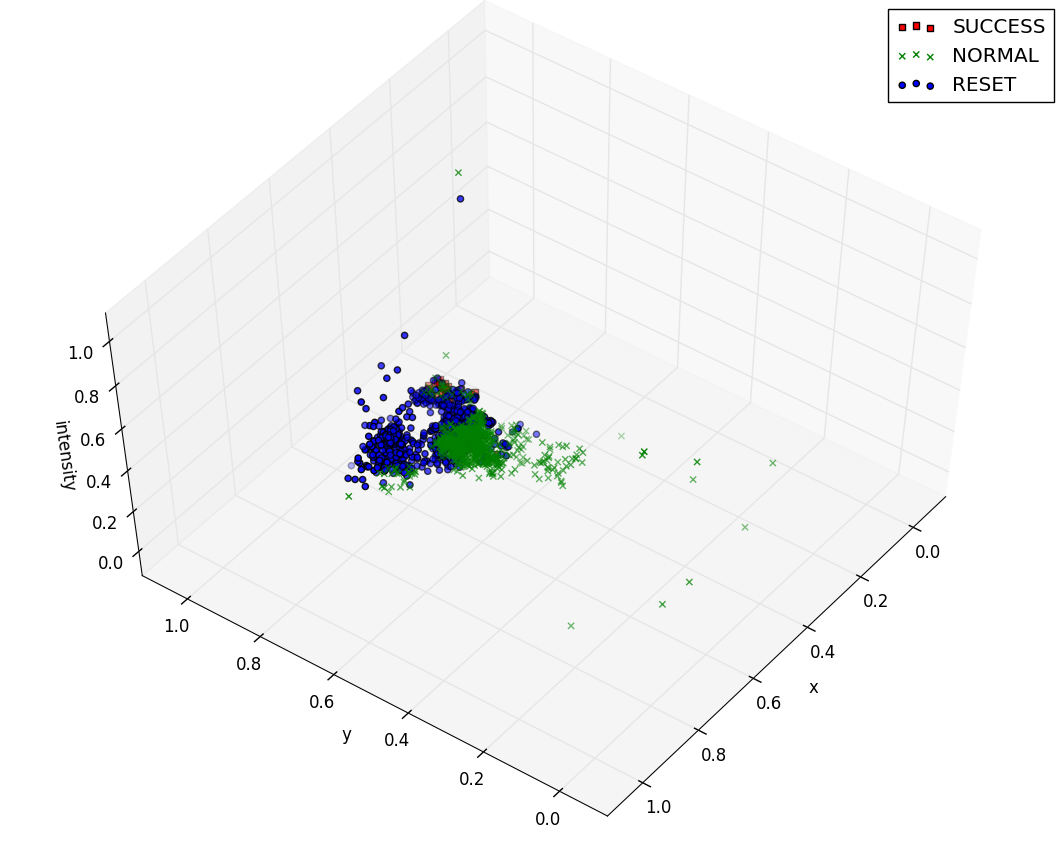
\includegraphics[width=\textwidth]{images/GA-binary-local.png}
    \caption{An example of the three-phase (GA + binary search + local search)
             algorithm.
    }
    \label{fig:three-phase-example}
\end{figure*}


In the general case where there are multiple blobs of unknown size, number,
and positioning with respect to each other, the situation is more complicated.
The problem of determining even how many blobs there are is nontrivial,
especially with a rather limited amount of information available. (Remember,
evaluations are expensive.) There is also the question of how to pick NORMAL
points so that no other blobs lie on the connecting line. A way to solve all
this would be to segment the search space in "BLOB" and "not BLOB" and so turn
it into a geometric problem, but again, the algorithm has limited information
at its disposal. The introduction of CHANGING points additionally muddles the
notion of the exact class border and brings in more hyperparameters. 

While this problem might be an interesting one to solve, it runs the risk of
becoming a significant piece of work by itself. With the given time constraints,
it seemed logical not to pursue this approach for the time being.
%I made the decision not to pursue this approach for the time being.
%I made the decision to prioritize other approaches.


\subsection{Some other variants}
Certain other variants were tried out or under trial: a simple particle swarm
optimization (PSO) algorithm, which turned out to be good at traversing the
parameter space, but would take many more iterations than was reasonable given
the expensive nature of point evaluation; one memetic algorithm, which interleaves
generations of the GA with local modification of the point was also on trial, but
its development was given low priority since it did not do too well in initial
testing.

\subsection{The variant used}
For the final version of the evolutionary algorithm, a variation on the
three-phase version was used; more specifically, the binary search phase
was thrown out, and the hyperparameters were set to values meant to ensure
a reasonable execution time of the algorithm -- the EA does not terminate
after a fixed number of evaluations, but the execution time depends on the
results it finds.

Additionally, the probe tip was replaced with a smaller, more precise one;
the result of this was that, on random scans, the share of faulty responses
fell almost fivefold, and the share of unique faulty responses slightly increased.
A similar effect occurred for the EA. This is expected: the probe affects not
a single point, but an area. Hitting a smaller area means that points otherwise
near, which would before have affected each other enough not to be distinguishable,
now produce a different effect.


\section{The results}\label{sec:results}
This section presents the results of injecting faults into SHA3-512.

%First, we investigate how well is GA able to find faults (i.e., force the algorithm
%to output the wrong ciphertext) and then, whether such points can be used in order
%to obtain the state of the algorithm.
%
%There, we use algebraic fault analysis (AFA), as described in~\cite{luo2018algebraic}.
%AFA eliminates the need for analysis of fault propagation as is needed in differential
%fault analysis; instead it uses a SAT solver to recover the state bits from a
%(clean output, faulty output) pair.

The duration of the EA is determined by the number of faults it finds.
Five independent runs were conducted, with 2\,074, 2\,343, 3\,353, 3\,606,
and 5\,132 points, respectively. Each individual run will be different due
to the stochastic nature of the algorithm, as well as of the target's response.
To obtain statistically meaningful results, the reported values are averages over all runs.
On average, in each run there are 3\,301.6 points, of which:
\begin{itemize}
	\item 662.8  (18.9\%) NORMAL
	\item 496.4  (15.0\%) RESET
	\item 375.2  (11.4\%) CHANGING
	\item 1\,807.2 (54.7\%) SUCCESS
\end{itemize}

This also means there are 16\,508 individual measurements on average.
Out of these, 9\,700.4 (58.8\%) are faulty, and 3\,288.4 (19.9\%) are unique/distinct.
Comparing this with random search with 3\,302 points, we get:
\begin{itemize}
	\item 2\,995.8 (90.7\%) NORMAL
	\item 65.0 (2.0\%) RESET
	\item 232.4 (7.0\%) CHANGING
	\item 8.8 (0.3\%) SUCCESS
\end{itemize}

Again, this would represent 16\,510 individual measurements.
Out of these, 228.2 (1.3\%) are faulty, and 160.8 (1.0\%) are unique/distinct.
To conclude, when averaged over 5 runs, the EA algorithm gives 42.5 times more faulty
measurements, and 20.5 times more distinct faulty ones.
The somewhat lower share of distinct measurements for the EA algorithm
can be explained by many SUCCESS points being close to each other due to the
local search phase, thus being more likely to cause the same response.

Tables~\ref{tab:500} until~\ref{tab:2000} contain results for the random search
and evolutionary algorithms when considering the first 500, 1\,000, and 2\,000
points, respectively. Note how the results for random search do not change
significantly with more measurements. At the same time, we see that the EA is
very successful already for the smallest case where with only 500 points,
and as we add more points, the percentage of SUCCESS points increases.

\begin{table}[!hbtp]
	\small
	\caption{500 points.}
	\label{tab:500}
	\centering
	\begin{tabular}{ccc}
		           &     Random     &       EA       \\ \toprule
		  NORMAL   & 452.6 (90.5\%) & 315.2 (63.0\%) \\
		  RESET    &  9.8 (2.0\%)   & 73.4 (14.7\%)  \\
		 CHANGING  &  36.0 (7.2\%)  & 79.0 (15.8\%)  \\
		 SUCCESS   &  1.6 (0.3\%)   &  32.4 (6.5\%)  \\ \midrule
		 \#faults  &  33.4 (1.3\%)  & 260.8 (10.4\%) \\
		\#distinct &  22.6 (0.9\%)  & 158.8 (6.3\%)  \\ \bottomrule
	\end{tabular}
\end{table}

\begin{table}
	\small
	\caption{1\,000 points.}
	\label{tab:1000}
	\centering
	\begin{tabular}{ccc}
		           &     Random     &        EA         \\ \toprule
		  NORMAL   & 910.4 (91.0\%) &  381.8 (38.2\%)   \\
		  RESET    &  19.6 (2.0\%)  &  198.0 (19.8\%)   \\
		 CHANGING  &  67.2 (6.7\%)  &  169.2 (16.9\%)   \\
		 SUCCESS   &  2.8 (0.3\%)   &  251.0 (25.1\%)   \\ \midrule
		 \#faults  &  58.8 (1.2\%)  & 1\,530.4 (30.6\%) \\
		\#distinct &  40.4 (0.8\%)  &  956.6 (19.1\%)   \\ \bottomrule
	\end{tabular}
\end{table}

\begin{table}
	\small
	\caption{2\,000 points.}
	\label{tab:2000}
	\centering
	\begin{tabular}{ccc}
		           &      Random       &        EA         \\ \toprule
		  NORMAL   & 1\,814.6 (90.7\%) &  541.6 (27.1\%)   \\
		  RESET    &   36.6 (1.8\%)    &  351.2 (17.6\%)   \\
		 CHANGING  &   144.2 (7.2\%)   &  285.0 (14.2\%)   \\
		 SUCCESS   &    4.6 (0.2\%)    &  822.2 (41.1\%)   \\ \midrule
		 \#faults  &   130.6 (1.3\%)   & 4\,606.4 (46.0\%) \\
		\#distinct &   93.4 (0.9\%)    & 2\,030.4 (20.3\%) \\ \bottomrule
	\end{tabular}
\end{table}


Finally, the search space after random search or EA is shown in Figures~\ref{fig:random1}
until~\ref{fig:ga3}. Figures~\ref{fig:random1} and~\ref{fig:ga1} give results
projected down onto the XY-plane, i.e. by just the X and Y parameters. Figures~\ref{fig:random2}
until~\ref{fig:ga3} depict depict intensity as a third parameter. For less clutter,
versions without NORMAL points are also provided. The number of points in case
of random search is always 3\,302; for the EA, the run with 3\,606 points is shown.
Naturally, figures without the NORMAL points have less points.

\begin{figure*}
	\centering
	\begin{subfigure}[b]{0.49\textwidth}
		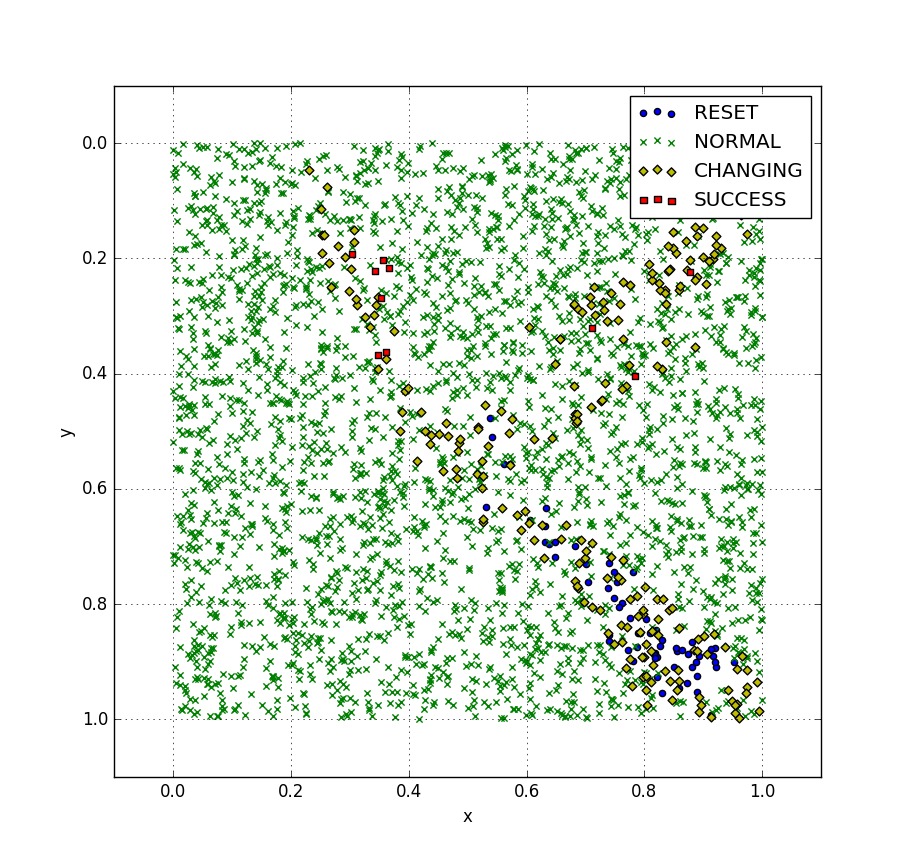
\includegraphics[width=0.98\linewidth]{images/plots/plot_random_2D.png}
		\caption{Random search in 2D}
		\label{fig:random1}
	\end{subfigure}
	\begin{subfigure}[b]{0.49\textwidth}
		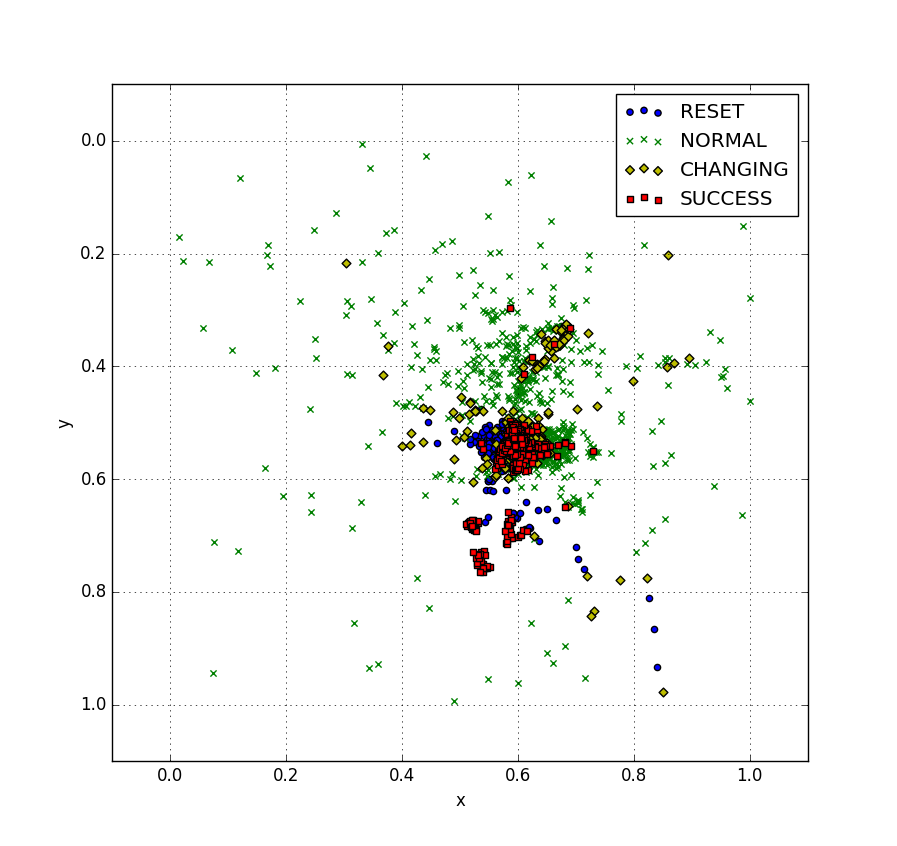
\includegraphics[width=0.98\linewidth]{images/plots/plot_GA_3_2D.png}
		\caption{GA and local search in 2D}
		\label{fig:ga1}
	\end{subfigure}
	\begin{subfigure}[b]{0.49\textwidth}
		\centering
		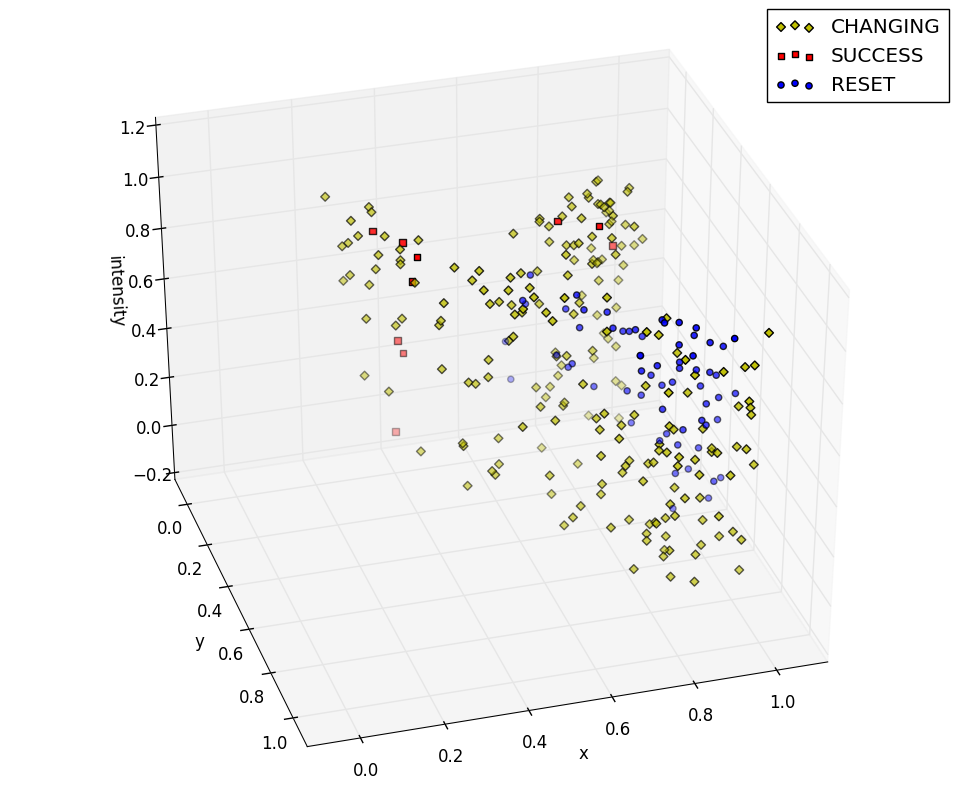
\includegraphics[width=0.98\linewidth]{images/plots/plot_random_3D_nonormal.png}
		\caption{Random search without NORMAL points}
		\label{fig:random2}
	\end{subfigure}		
	\begin{subfigure}[b]{0.49\textwidth}			
		\centering
		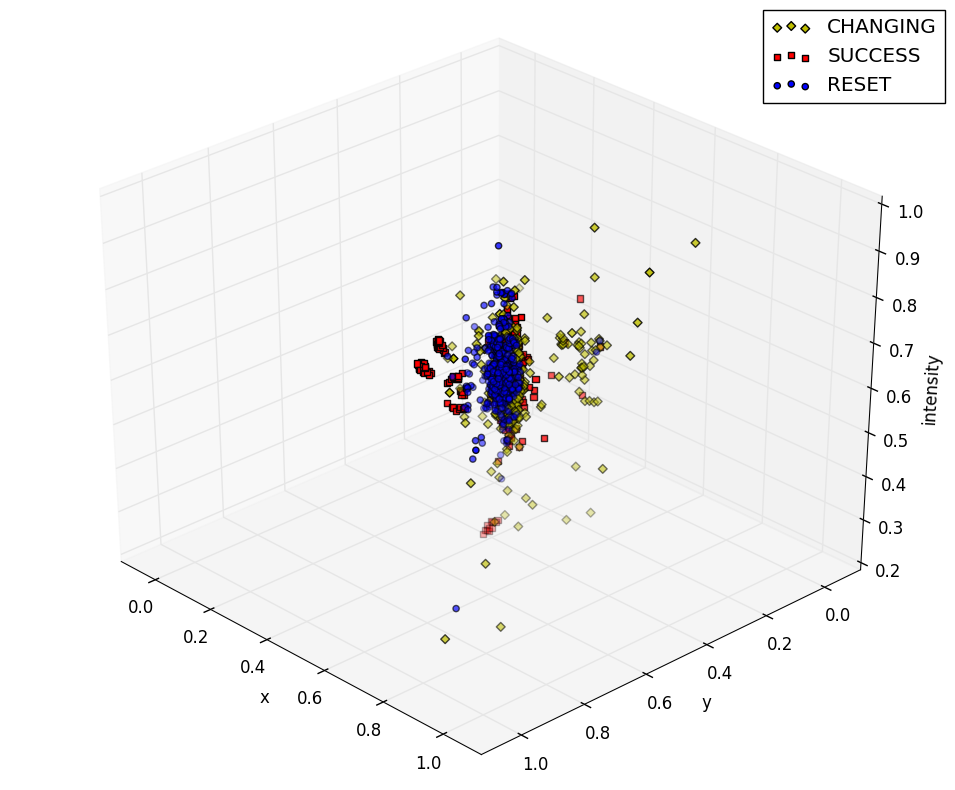
\includegraphics[width=0.98\linewidth]{images/plots/plot_GA_3_3D_nonormal.png}
		\caption{GA and local search without NORMAL points}
		\label{fig:ga2}
	\end{subfigure}
	\begin{subfigure}[b]{0.49\textwidth}
		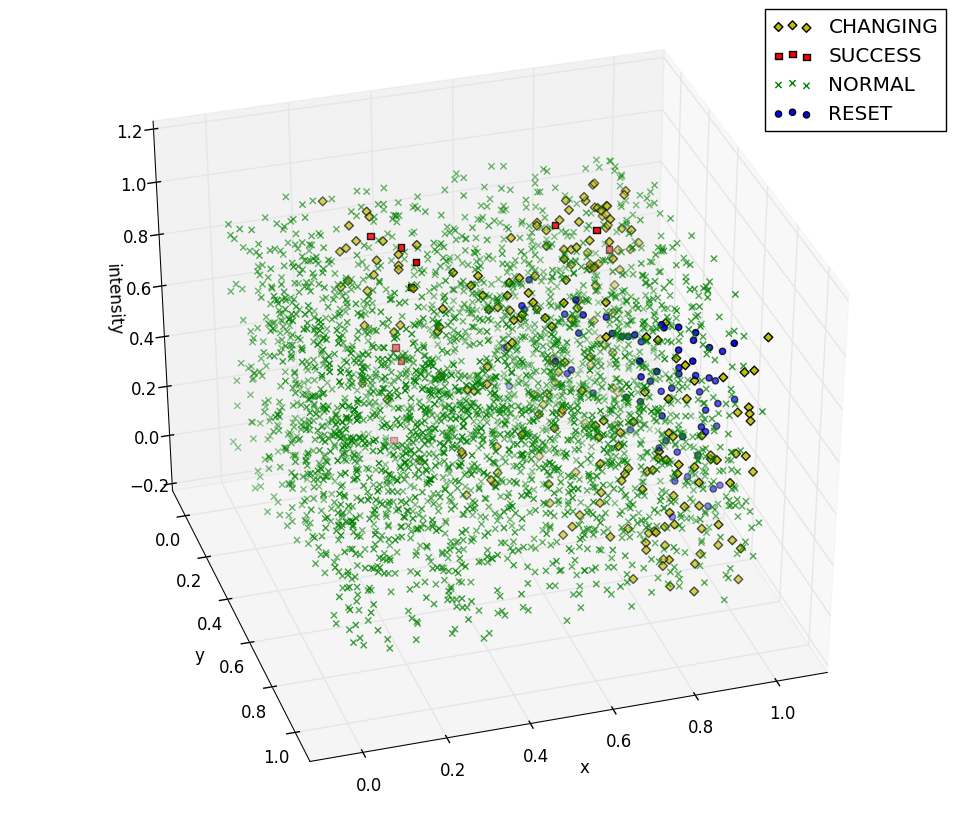
\includegraphics[width=0.98\linewidth]{images/plots/plot_random_3D.png}
		\caption{Random search}
		\label{fig:random3}
	\end{subfigure}
	\begin{subfigure}[b]{0.49\textwidth}
		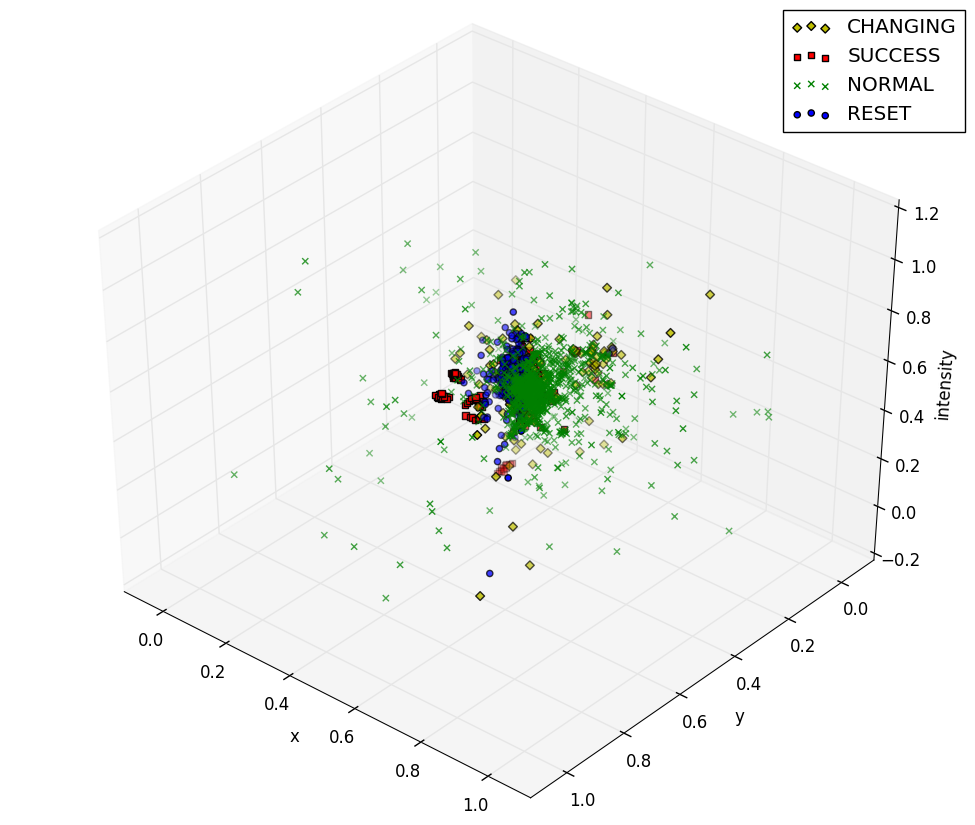
\includegraphics[width=0.98\linewidth]{images/plots/plot_GA_3_3D.png}
		\caption{GA and local search}
		\label{fig:ga3}
	\end{subfigure}
	\label{fig:figures}
	\caption{Results for EA (GA with local search) and random search.}
\end{figure*}




\chapter{Attacking SHA-3}\label{ch:attacking_keccak}
The ultimate goal of optimizing fault injection parameters is, of course, to
do fault injection attacks. This chapter presents exactly that: a fault attack
on SHA-3 (specifically, SHA3-512) in practice.

\section{State of the art}
To the best of my knowledge, no implementation of SHA-3 has yet been attacked in
practice. The attacks which do exist are only simulated:~\cite{DFA_SHA-3_single-bit}
show that differential fault analysis (DFA) can be used to recover the complete
state in around 80 faults on average, if the attacker is able to inject single-bit
faults in the input of the penultimate round (i.e. $\theta^{22}_i$), though they
rely on brute-forcing the last few bits. According to~\cite{luo2017relaxed}
(itself an extension of~\cite{luo2016shortSHA3}), this is around 500 single-bit
random faults for the whole state. In \cite{luo2017relaxed}, the attack is
generalized to a single-byte fault model, recovering the state in around 120
random faults.

Algebraic fault analysis (AFA) is more promising: in the progress
through~\cite{luo2016shortSHA3},~\cite{luo2017relaxed}, and~\cite{luo2018algebraic},
the authors manage to bring down the number of faults needed to recover the
internal state with SHA3-512 down to under 10 with AFA and the 32-bit fault
model.

Besides being more efficient at recovering state, AFA has several advantages:
\begin{itemize}
 \item It does not require analysis of fault propagation through the algorithm,
       making it much easier to abstract the internal details.
 \item The fault model can be easily changed, by just changing the appropriate constraints.
 \item Perhaps most importantly, it works for more relaxed fault models.
\end{itemize}


\section{Description of the attack}
The attack used here is the one in~\cite{luo2018algebraic}.
Again, like the other papers concerning fault injection into Keccak, it requires
the attacker to be able to inject multiple faults in the input of round 22 of Keccak.
These faults are allowed to affect up to 1 unit of the state, where units are sized
8b, 16b, or 32b, depending on the fault model. This means that, for example, with
a 32-bit fault model and the internal state $A[200]$, the fault model allows us
to fault bytes $A[0]$ through $A[3]$ inclusive, but not bytes $A[1]$ through $A[4]$,
since that crosses the line between two 32-bit units ($A[0]$ to $A[3]$ is the first
such unit, $A[4]$ to $A[7]$ the second, etc.).

The Keccak permutation, by virtue of being a permutation, is invertible.
The same applies to its individual rounds. This means it is enough to recover
the entire state at \emph{some} point in the execution. As in previous work, the
chosen target state is $\chi^{22}_i$, the input to the nonlinear $\chi$
transformation of round 22.
For state recovery, we reused their C++ retrieval code (which uses CryptoMiniSAT
for SAT solving).

The general idea behind AFA on SHA-3/Keccak is simple: use a SAT solver to do
the work for us: all we need is to provide appropriate constraints for it.
We start with 1\,600 Boolean variables representing the state ($\theta^{22}_i$)
and then provide constraints:
\begin{description}
    \item[Fault Model] -- what kind of a fault do we cause?\\
	There's a separate set of (up to) 1\,600 Boolean variables ($\Delta\theta^{22}_i$)
    representing the induced fault. $\theta^{22}_i \oplus \Delta\theta^{22}_i$ is the
    faulted state, before propagating through the final two rounds of the algorithm.
	Depending on what the fault model is, we add constraints such as ``exactly one bit
    of $\Delta\theta^{22}_i$ is non-zero'', corresponding to a one-bit fault model, or
    slightly more verbose ones for specifying things such as ``we faulted a word-aligned
    32-bit word'', which would correspond to a 32-bit fault model in~\cite{luo2018algebraic}.

    \item[Keccak] -- how does the (faulted) internal state propagate?\\
	For Keccak, the internal transformations can be relatively simply encoded as Boolean expressions.
	This implicitly tells the solver everything it needs to know about fault propagation, regardless of
	the fault model constraints. There are two cases we consider:
	\begin{equation*}
	H= \iota^{23} \circ \chi \circ \pi \circ \rho \circ \theta \circ
	\iota^{22} \circ \chi \circ \pi \circ \rho \circ \theta(\theta^{22}_i)
	\end{equation*}
	where $H$ is the correct hash output, and
	\begin{equation*}
	H'= \iota^{23} \circ \chi \circ \pi \circ \rho \circ \theta \circ
	\iota^{22} \circ \chi \circ \pi \circ \rho \circ \theta(\theta^{22}_i \oplus \Delta\theta^{22}_i)
	\end{equation*}
	where $H'$ is the faulty hash output.

    \item[Outputs] -- which are the concrete outputs?\\
	We give the SAT solver the actual values of $H$ and $H'$.
	After so constraining the SAT solver, we can let it find a solution -- an
    internal state satisfying all the constraints. Once it finds the first such solution,
    we ban this newly-found solution by adding it as an additional constraint, and let the
    SAT solver find another one. This process is repeated until no new solutions can be found.
	
	The bits of the state which are the same in all solutions are the ones we can recover;
    as for those which take different values in different solutions, their values are
    not entailed by the combined constraints of the fault model, the algorithm, and
    the outputs (i.e. the ``real'' constraints).
	
	Depending on the fault model and the version of SHA-3 (SHA3-512, SHA3-224, etc.),
    these constraints may or may not be enough to recover part of the state. If this happens,
    additional constraints can be introduced, such as using \emph{two} faulty hashes at a time,
    $H'_1$ and $H'_2$, at a cost of having extra Boolean variables, making the problem harder
    for the SAT solver (this is Method II from~\cite{luo2018algebraic}); or, if we can first
    somehow recover part of the $\chi^{23}_i$ bits, we can use them to additionally constrain
    the SAT solver (this is Method III from~\cite{luo2018algebraic}).
\end{description}

As for the choice of fault model and method: 32-bit fault model and Method III
from~\cite{luo2018algebraic} was chosen. While the standard approach (Method I
-- single faulty output, no extra $\chi^{23}_i$ bits) approach would be preferable,
it is not possible according to the authors, at least when using two (and not more)
faults at once. In principle, there is no limit on the number of faults we can use
to constrain the SAT solver, but increasing this number quickly brings us where
running the solver is \emph{very} hard, and obtaining another exploitable fault
is cheaper than the extra SAT solving.
The main reason for choosing the 32-bit fault model was, the fact that the target
board has a 32-bit word size. This also being the most relaxed fault model means
that any 8-bit or 16-bit faults do not go to waste, but are also exploited.

%TODO: make copy of Table IV here?
Table IV in~\cite{luo2018algebraic} neatly presents what is possible in
reasonable time with the current state of the art in SAT solving: going from
longer-output SHA-3 functions to shorter-output ones, less information is
available to us, and state retrieval becomes progressively harder.
For SHA3-512 in particular, Method I is still usable in the 8-bit and 16-bit
fault models, requiring 45 and 23 faults on average to recover the state.
The 32-bit fault model requires using at least Method II; this comes at a
substantial cost in SAT solving time, but also a reduction in the number of
faults needed: on average 7 faults for Method II, and 6 for Method III.
Intuitively, this is because a fault can only leak so much information;
so we need either more faults, or larger faults.

With the 32-bit fault model, each fault usually allows the recovery of hundreds
of bits, according to~\cite{luo2018algebraic}. With Method II the distribution
is bimodal, with a part of faults allowing for $<$100 bits, and the rest around
500 bits; with Method III the lower mode vanishes, and the upper one stays
more-or-less where it is. We can conclude that, while the addition of extra
$\chi^{23}_i$ bits does make a difference in the total number of faults required,
it is not large. What is \emph{does} do, however, is drastically reduce the time
needed for retrieval --- by an order of magnitude.

This is the main reason for choosing Method III: it lets us approximate Method II,
with a \emph{lot} less computing power.
Since many more faults were generated for the purposes of this thesis than is
necessary for a single successful attack, great efficiency was needed to check
them all for exploitability.
So, the following method was used:
\begin{enumerate}
    \item obtain the bottom 640 bits of Keccak state ($\chi^{23}_i(X,0,Z)$
          and $\chi^{23}_i(X,0,Z)$), not by performing a separate recovery
          phase, but by using \texttt{memcpy()}
    \item generate a single faulty hash that is known to be the result of a
          good fault (in the 32-bit fault model); this is $H'_1$
    \item take a faulty hash generated by the real board; this is $H'_2$
    \item add those hashes as constraints and run the SAT solver
\end{enumerate}

If the recovery is unsuccessful, this means that the candidate hash $H'_2$ was
not an exploitable one. This method allows a $O($number of faults to test$)$
time complexity, which is absolutely needed to check the thousands of faults
obtained.


\section{Results obtained}
The exploitability of all distinct faulty hashes obtained by the evolutionary
algorithm, as well as of all those obtained by the random scan, was tested.
While the share of distinct/unique faulty hashes depends on the size of the scan,
the exploitability of a faulty hash does not. For this reason, I calculated the
share of exploitable individual faults on all the samples obtained (with the
same hyperparameters).


The results are as follows:
the EA generated a total of 14\,979 distinct faults (out of 82\,540 individual
measurements); 106 of these were exploitable 32-bit faults, for a share of 0.71\%.
Random search generated 947 distinct faults (out of 100\,000 individual
measurements); 110 of these were exploitable 32-bit faults, for a share of 11.61\%.
When translated into exploitable faults per individual measurement, this gives
about $1.41 \times 10^{-3}$ and $1.13 \times 10^{-3}$ for EA and random
search, respectively -- an improvement of 24.6\%.

Despite the fact that the EA is still significantly more successful than random search,
we see that actually most of the faults obtained with the EA cannot be translated into
exploitable faults. This results in a decrease between the performance difference
of the EA and random search. Still, such results are not entirely unexpected:
the EA was given no information on the exploitability of a fault that it could
use to guide its search. This could be addressed by having its fitness function
integrate an analysis of fault exploitability.



\chapter{Conclusion}\label{ch:conclusion}
In the end, the developed algorithm did not turn out to be really complex,
partly due to the short development schedule; however, even though fault injection
is widely used, the amount of work on its parameter optimization is surprisingly
small, and plenty of work still needs to be done. It is therefore not particularly
surprising that the developed algorithm ended up being substantially better than
the baseline: over 20 times more distinct faults per individual measurement than
random search; and almost 25\% more exploitable faults compared to random search.

To my knowledge, there is presently only one other method for EMFI parameter
optimization, the one given in~\cite{madau2017fault}, and described in section~\ref{sec:related_work}.
However, they consider RESET points to also be \emph{faults} worth preserving,
meaning we cannot do a direct comparison -- their task appears to be an easier one.
But if we look at their best case -- keeping 80\% of the faults while rejecting
75\% of the chip surface -- this is an increase in fault concentration by a
factor of merely 3.2, for a price of a full 2-dimensional grid scan.
Considering that the EA developed here likely runs in a comparable amount of time,
it is evident that their EMFISC approach is, as it stands, inferior.

Since there are few works looking at FI parameter optimization, there is a
number of potentially interesting research topics. The most obvious one is
certainly adding exploitability analysis to the fitness function -- filtering
out the non-exploitable SUCCESS points would be a great improvement to this
algorithm. I expect that making it run in real-time on a single workstation
would not be easy. One less obvious follow-up topic would be: what is a
neighbourhood? A way to figure out the effective lowest resolution would
potentially make the search space considerably smaller.

And, of course, this algorithm should be tested on other boards as well.
As it turns out, there are good reasons why this particular board is named
the \emph{Piñata}: one, it is fairly susceptible to being exploited by various
means; this makes it an excellent practice target for fault injection.
Two, like the real thing, it is meant to take a beating: millions of glitches,
day in, day out. This second reason is why it was chosen -- nobody wants a dead
board in the middle of a five-day scan -- but the first reason might be the cause
for what seems an unusually high number of faults in total.




\bibliography{literatura}
\bibliographystyle{fer}

\begin{sazetak}
Kriptografija je u temeljima velikog dijela moderne računalne infrastrukture,
stoga je vrlo bitno da se u nju možemo pouzdati. Sigurnost malih, ugradbenih
uređaja čini jedan dio tog. \\
Elektromagnetsko umetanje greške (EMFI) je moćna tehnika za izvođenje napada
umetanjem pogreške, ali zahtijeva odabir dobrih parametara u prostoru daleko
prevelikom da bi se mogao iscrpno pretražiti. U ovom radu se iznosi evolucijski
algoritam za pretragu prostora parametara za umetanje greške, kao i logika
iza njegovog razvoja. Ovaj algoritam se potom koristi za pronalazak grešaka
koje se koriste za algebarsku analizu grešaka (AFA) na SHA-3 (Keccak)
kriptografskom heš algoritmu; dana je usporedba rezultata sa slučajnom
osnovicom.

\kljucnerijeci{umetanje pogreške, evolucijski algoritam, SHA-3, algebarska analiza grešaka, optimizacija parametara}
\end{sazetak}

\pagebreak
\begin{abstract}
Cryptography underpins a large part of modern computer infrastructure, making
its reliability very important. The security of embedded devices and their
tamper-resistance is a small part of this. \\
Electromagnetic fault injection (EMFI) is a powerful fault injection technique
for conducting fault injection (FI) attacks, however it requires choosing
parameters in a parameter space that's far too large to perform an exhaustive
search, and presently there appears to be no good method for conducting the
search for good parameters. In this thesis, an evolutionary algorithm for FI
parameter search is presented, along with the rationale used in its development.
This algorithm is used to find faults for an algebraic fault attack (AFA) on the
SHA-3 (Keccak) cryptographic hash algorithm, and its results are compared with
the random baseline.

\keywords{electromagnetic fault injection, evolutionary algorithm, SHA-3, algebraic fault attack, parameter optimization}
\end{abstract}

\end{document}
